\chapter[Embasamento Teórico]{Embasamento Teórico}

\label{chap:embasamento_teorico}

Neste capítulo, são apresentados os principais conceitos utilizados para embasamento da ferramenta desenvolvida, sendo essa focada na Engenharia de Requisitos e suas principais atividades/etapas. Primeiramente, terá uma seção descrevendo, de forma mais conceitual e abrangente, a Engenharia de Requisitos (Seção \ref{sec:eng_requisitos_ex}). Logo em seguida, será apresentado o tópico de Rastreabilidade (Seção \ref{sec:rastreabilidade}), definindo conceitos importantes no domínio da Engenharia de Requisitos. Serão apresentadas as técnicas referentes ao tópico de Elicitação (Seção \ref{sec:elicitacao}). Adicionalmente, será apresentada uma seção sobre Modelagem (Seção \ref{sec:modelagem}), definindo os principais modelos para a ferramenta. Posteriormente, têm-se os tópicos de Verificação (Seção \ref{sec:verificacao}) e Priorização (Seção \ref{sec:priorizacao}). Logo em seguida, têm-se as definições de \textit{House of Quality} (Seção \ref{sec:house_of_quality}), bem como as definições de Grafos, fundamentais para a ferramenta. Por fim, tem-se o resumo do capítulo (Seção \ref{sec:resumo_embasamento}). Como há um vasto conjunto de conceitos, a Figura \ref{fig:roadmap} confere um roteiro de leitura, procurando auxiliar na compreensão do conteúdo exposto.

\begin{figure}[]
    \begin{center}
        \caption{Infográfico do Processo da Ferramenta}
        \label{fig:roadmap}
        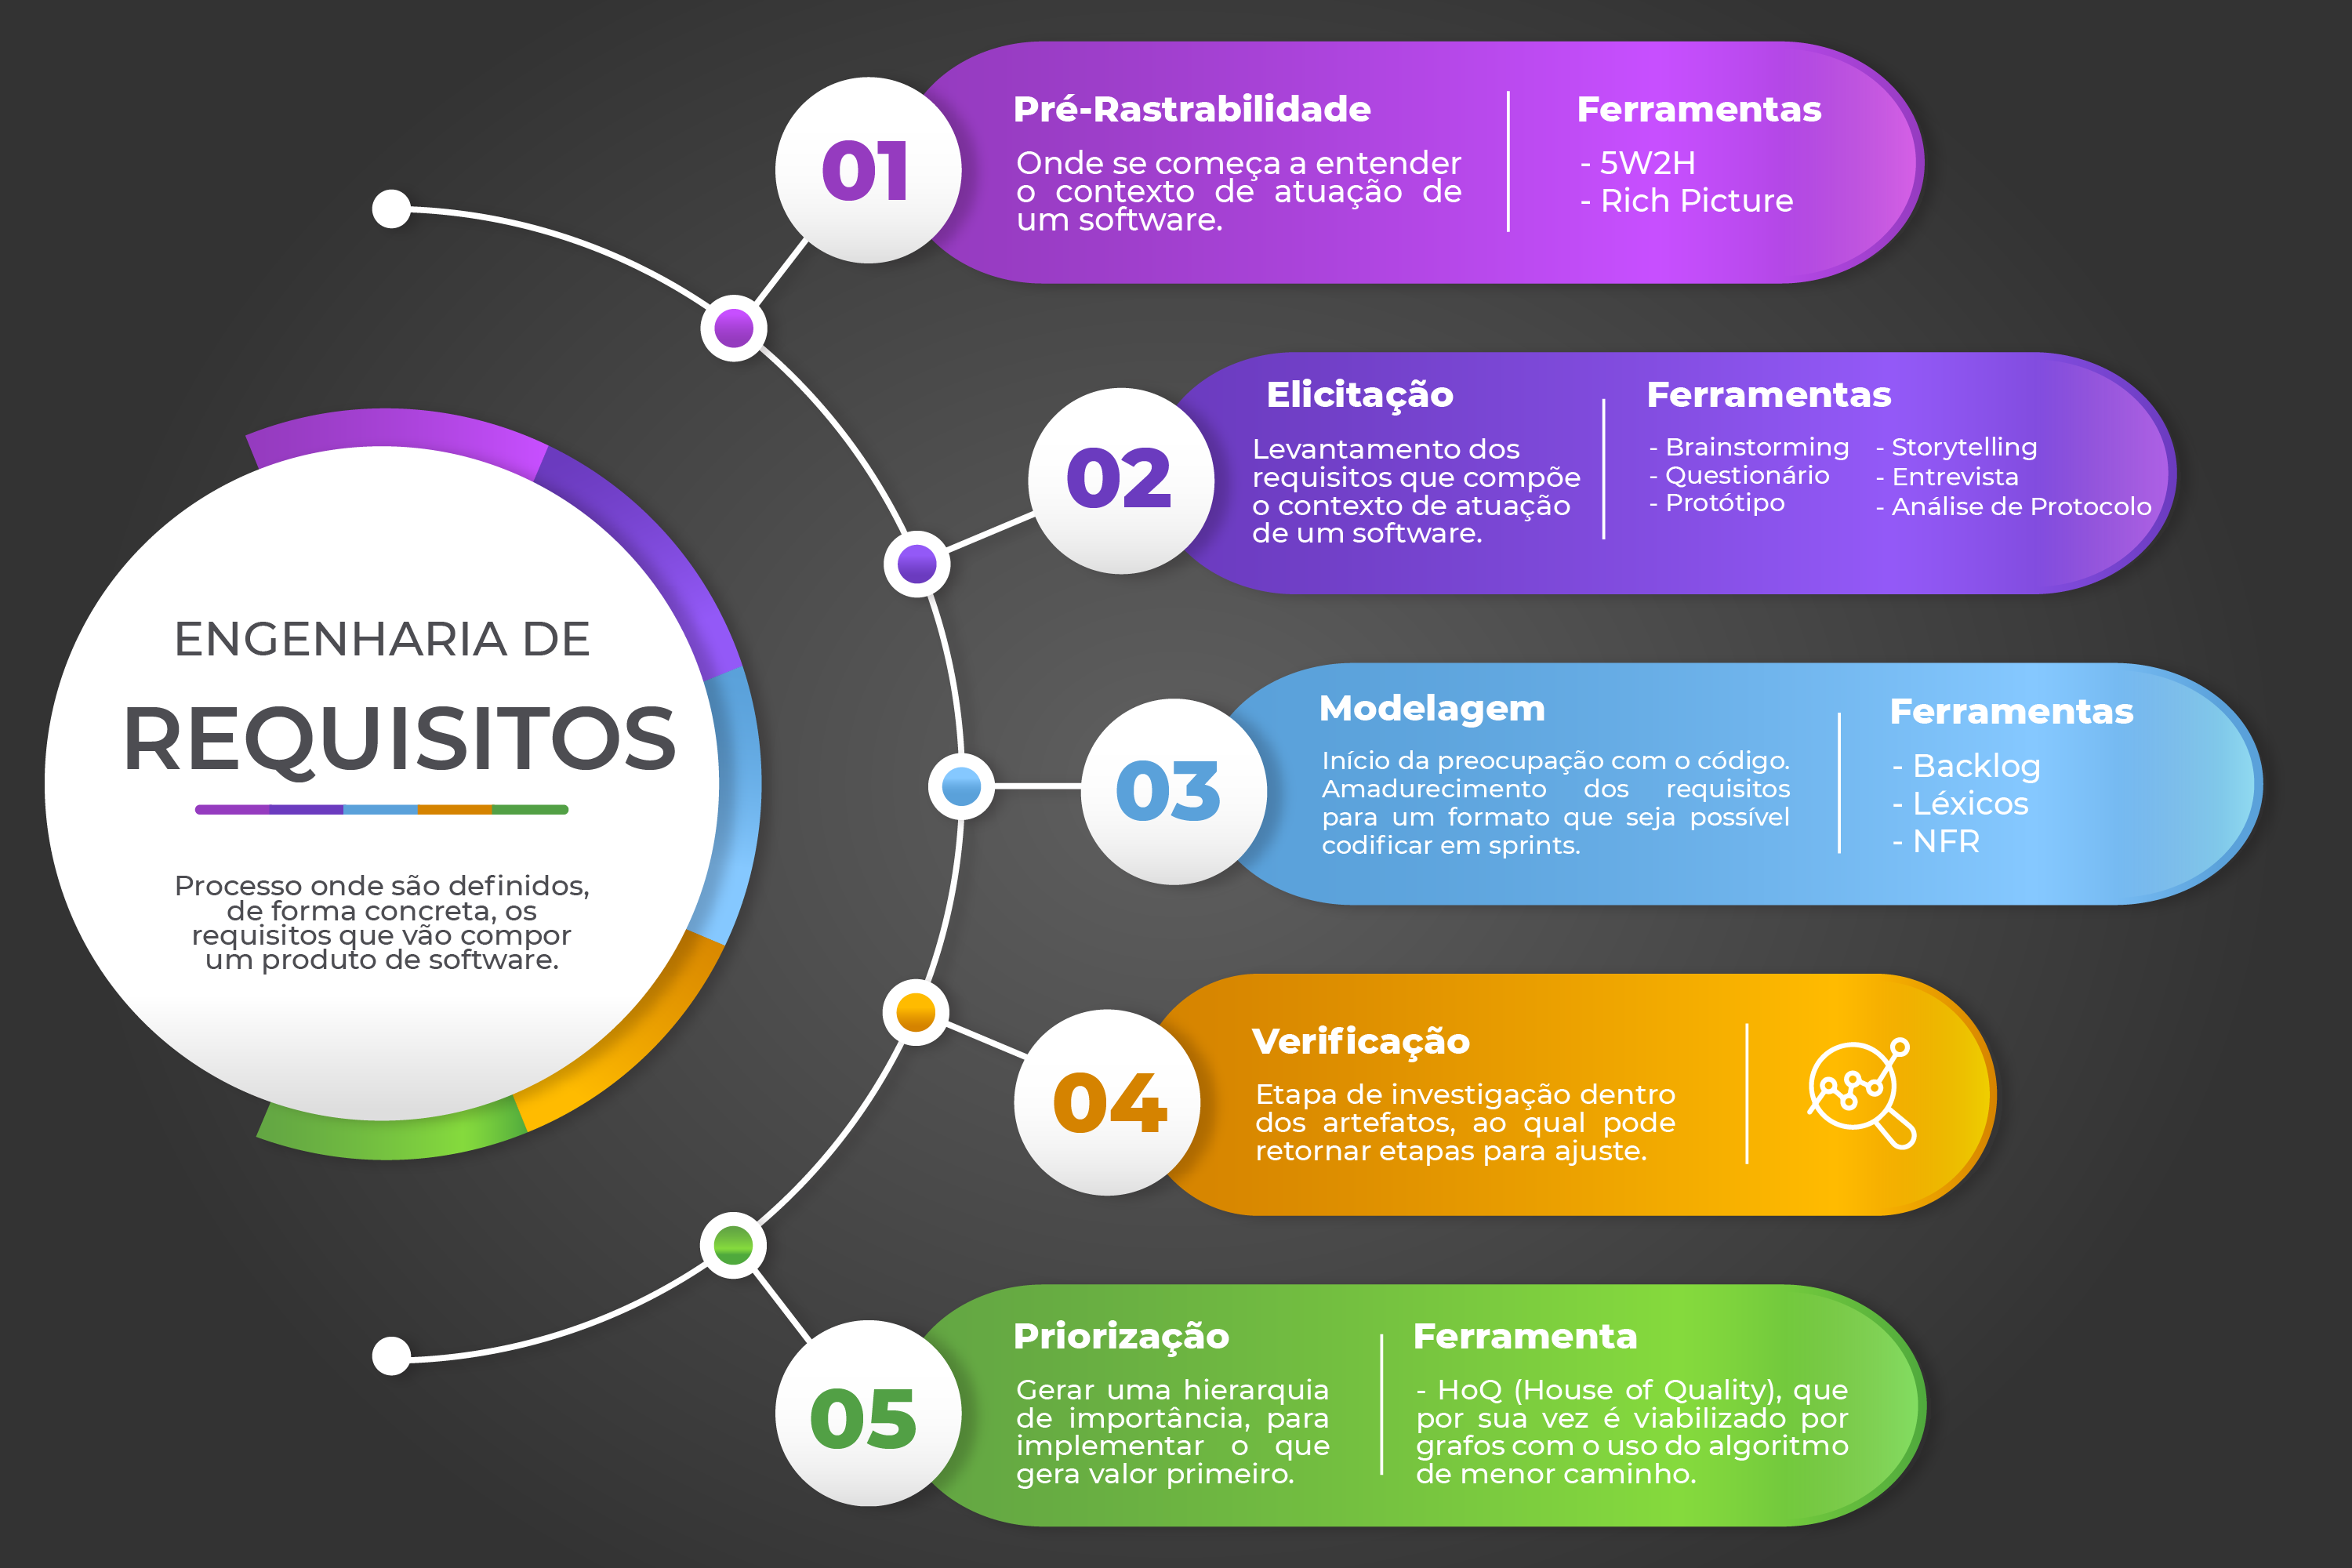
\includegraphics[scale=0.58]{figuras/Embasamento/infografico_engenharia_requisitos.png}
        \legend{Fonte: Autores, 2022.}
    \end{center}
\end{figure}

A macro área de interesse deste trabalho é a Engenharia de \textit{Software}. A ferramenta desenvolvida compreende, como principal ponto, contribuições no escopo da Engenharia de Requisitos, que será mais bem detalhada ainda nesse capítulo, mas que trata da etapa que define concretamente os requisitos que vão compor um produto de \textit{Software}.

Nesse contexto, para a ferramenta desenvolvida, foram escolhidas algumas etapas de maior relevância para que se tenha um processo mais certeiro na elaboração de um novo produto de \textit{software} com qualidade e os artefatos (documentos) usados para tanto. São eles:

\begin{itemize}
    \item Pré-rastreabilidade: para viabilizar esta atividade, podem ser utilizados diferentes artefatos, sendo sugeridos, no contexto desse trabalho: \textit{Rich Picture} (Seção \ref{sec:rich_picture}) e \textit{5W2H} (Seção \ref{sec:5w2h}). Esta etapa viabiliza um olhar mais centrado no que tange o contexto de uma aplicação, permitindo esboçar as primeiras ideias em artefatos de cunho mais generalista, e livres de notação formal. Adicionalmente, permite manter um elo, por exemplo, para as fontes de informação;
    
    \item Elicitação: para condução desta atividade, há técnicas bem estabelecidas, tais como: \textit{Brainstorming} (Seção \ref{sec:brainstorming}), Questionário (Seção \ref{sec:questionario}), Prototipação (Seção \ref{sec:prototipo-def}), \textit{Storytelling} (Seção \ref{sec:storytelling}), Entrevista (Seção \ref{sec:entrevista}) e Análise de Protocolo (Seção \ref{sec:analise-protocolo}). Neste trabalho, são apresentadas breves definições sobre cada técnica. A partir das técnicas propostas, o principal objetivo é levantar as funcionalidades (requisitos funcionais e não funcionais) de uma aplicação de \textit{software};
    
    \item Modelagem: olhar mais centrado em fazer com que as ideias levantadas na etapa anterior tenham um aspecto mais maduro e que possam ser, de fato, implementado em código. Nesse contexto, existem vários níveis e propostas de modelagem. Entretanto, há ênfase em alguns artefatos, os quais corroboram com a modelagem em diferentes aspectos de um \textit{software}. O \textit{Backlog} do Produto (Seção \ref{sec:backlog}) permite especificar os requisitos funcionais de um \textit{software}, sendo um artefato muito conhecido e orientado às metodologias ágeis. O \textit{Softgoal Interdependence Graph} (SIG) compreende uma modelagem centrada em requisitos não funcionais, sendo proposta em um \textit{framework} conceitual conhecido como NFR \textit{Framework} (Seção \ref{sec:nfr}). Além disso, os Léxicos (Seção \ref{sec:lexicos}) são relevantes para compreensão dos principais termos de um produto de \textit{software}, sejam esses de cunho mais técnico ou de um domínio particular;
    
    \item Verificação: Para realização desta atividade, deve-se ter em mente as práticas de Verificação e Validação (Seção \ref{sec:verificacao}). Esta etapa visa encontrar erros e inconsistências nos modelos e requisitos levantados;
    
    \item Pós-rastreabilidade: O olhar desta atividade concentra-se em manter elos entre requisitos e artefatos de níveis mais baixos de abstração (Arquitetura e Código). Nesse ponto, o principal objetivo, é prover um rastro do requisito desde a sua primeira concepção, e
    
    \item Priorização/\textit{House of Quality} (Seção \ref{sec:priorizacao} e \ref{sec:house_of_quality}): etapa que visa definir qual a ordem que os requisitos devem ser implementados, que gere maior valor para os seus \textit{Stakeholders}. Acorda uma modelagem gráfica, que tem em vista correlacionar as preocupações entre diferentes \textit{Stakeholders}, sendo muito útil para lidar com interesses conflitantes e visualizar as funcionalidades que são mais relevantes, dados os aspectos qualitativos (requisitos não funcionais) do \textit{software}.
    
\end{itemize}

Cabe colocar que a ferramenta desenvolvida orienta o desenvolvimento de um Produto Mínimo Viável de \textit{software}, considerando a Engenharia de Requisitos e suas atividades. Neste sentido, algumas automatizações são realizadas, demandando estabelecer e se apoiar no conceito de um \textit{Minimum Viable Product} (MVP), em sua versão preliminar.

Diante da necessidade de se prover um MVP, e orientando-se pelas etapas e artefatos mencionados anteriormente, em especial pela priorização do \textit{House of Quality}, foram automatizadas algumas partes deste processo. Tendo em vista a \textit{House of Quality} e suas relações finalizadas, é utilizado o conceito de um Grafo, bem como o Algoritmo de Menor Caminho para a geração do MVP, em sua versão preliminar.

\section{Engenharia de Requisitos}

\label{sec:eng_requisitos_ex}

Por se tratar de uma área que se encontra entre o abstrato e o concreto, \citeonline{westfall_5w2h}, em seu estudo, define os diferentes porquês da existência da Engenharia de Requisitos, sendo:

\begin{itemize}
    \item O que é?: são os requisitos responsáveis pela definição do que o \textit{software} deve realizar (\textit{requisitos funcionais}\footnote{Declarações de serviços que o sistema deve prover, como tem que reagir para entradas e como precisa se comportar em situações especificas \cite{Sommerville10}.}) e possuir (\textit{requisitos não funcionais}\footnote{Restrições aos serviços ou funções oferecidas pelo sistema. Aplicam-se ao sistema na totalidade \cite{Sommerville10}.}) para agregar valor para os seus \textit{stakeholders}\footnote{Grupo de pessoas interessadas no produto, podendo ser cliente, usuários etc.}; Existem vários níveis e categorias de requisitos, mostrados na Figura \ref{lev_tipo_req}.
    
    \begin{figure}[htb]
        \begin{center}
            \caption{Níveis e Categorias de Requisitos}
            \label{lev_tipo_req}
            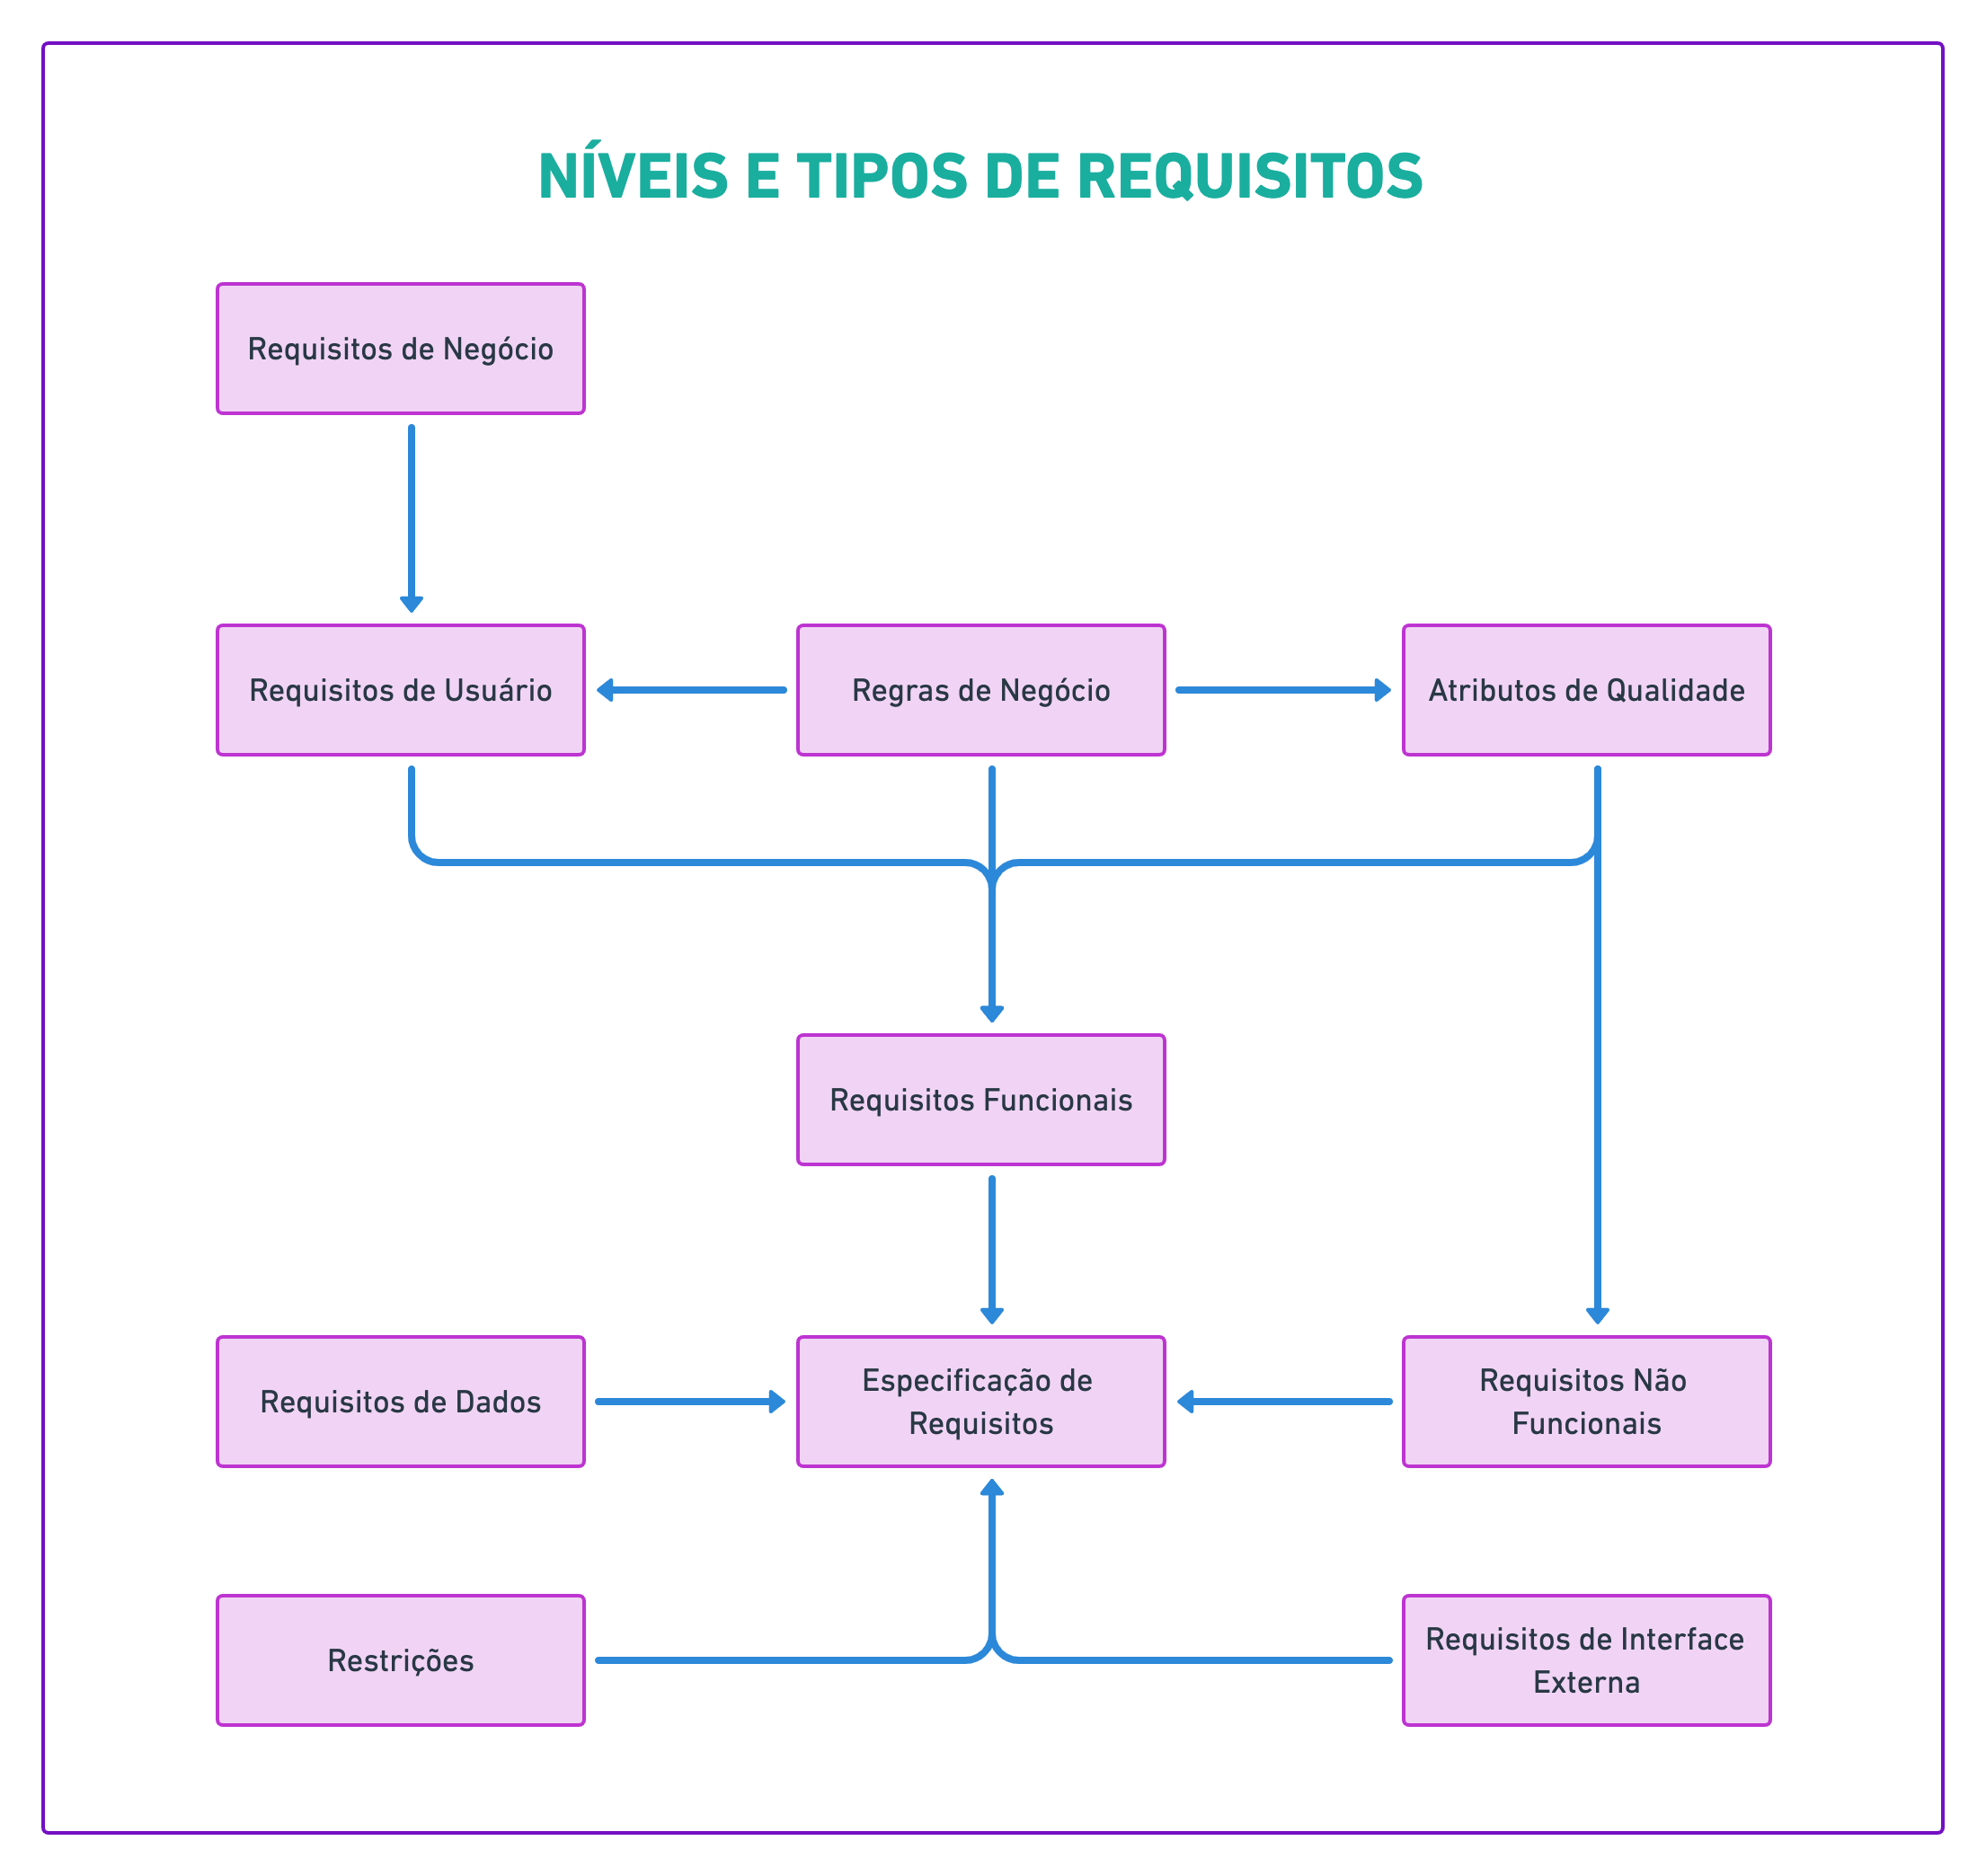
\includegraphics[scale=0.15]{figuras/Embasamento/lev_tipo_req.png}
            \legend{Fonte: \citeauthoronline{westfall_5w2h}, \citeyear{westfall_5w2h}}
        \end{center}
    \end{figure}
    
    \begin{itemize}
    
        \item Os \textbf{requisitos de negócio} definem, diretamente, quais são os problemas que devem ser resolvidos e porque o produto de \textit{software} está sendo desenvolvido;
        
        \item Os \textbf{requisitos de usuário} têm o objetivo de visualizar as funcionalidades do produto de \textit{software} a partir da perspectiva do usuário. Resumidamente, eles definem o que o \textit{software} deve realizar para que os usuários atinjam seus objetivos;
        
        \item Os \textbf{requisitos funcionais} de produto definem as funcionalidades do \textit{software} que devem ser implementadas para que os usuários consigam realizar suas tarefas de forma fácil;
        
        \item As \textbf{regras de negócio} são declarações sobre a forma da empresa fazer negócio, ou seja, elas refletem as políticas, os padrões, as práticas, os regulamentos e as diretrizes de negócio;
        
        \item Os \textbf{atributos de qualidade} no nível de usuário delimitam requisitos não funcionais que determinam o produto de \textit{software}. Incluem confiabilidade, disponibilidade, segurança, manutenibilidade, portabilidade, usabilidade, dentre outros;
        
        \item Os \textbf{requisitos de \textit{interface} externa}, objetivamente, definem o fluxo de informações através de \textit{interfaces} compartilhadas;
        
        \item As \textbf{restrições} têm o objetivo de mostrar quais destas limitações foram colocadas pelo fornecedor ao projetar e desenvolver o \textit{software}, e
        
        \item Os \textbf{requisitos de dados} definem os itens de dados específicos que devem ser introduzidos como parte do produto de \textit{software}.
    
    \end{itemize}
    
    \item Para que serve? : um dos grandes nomes da Engenharia de \textit{Software}, \citeauthoronline{brooks1995mythical}(\citeyear{brooks1995mythical}), afirma que:
        \begin{citacao}
            A parte mais difícil da construção de um sistema de \textit{software} é decidir precisamente o que deve ser feito. Nenhuma outra parte do trabalho conceitual é tão custosa quanto estabelecer detalhadamente os requisitos técnicos, incluindo todas as interfaces para os usuários, para os computadores, e para os outros sistemas do \textit{software}. Nenhuma outra parte do trabalho prejudica tanto o sistema se for feita de maneira errada. Nenhuma outra parte é tão difícil de ser retificada posteriormente.
        \end{citacao}
    Assim, pode-se entender o quão crítica é essa fase do processo de desenvolvimento de \textit{software}, contexto que se insere esse trabalho.
    
    \item Para quem?: os \textit{stakeholders} são indivíduos que impactam ou que são impactados pelo produto de \textit{software}. Portanto, possuem um nível de influência sobre o produto. Dentro desse contexto, existem diferentes perspectivas relacionadas à atuação de cada indivíduo, sendo as mais comuns:
    
    \begin{itemize}
        \item Os Analistas de Requisitos são essenciais dentro dessa área pelo fato deles serem responsáveis pela elicitação, análise e especificação dos requisitos, além de comunicarem as necessidades aos desenvolvedores e às partes interessadas;
    
        \item Os Arquitetos de \textit{Software} são essenciais por criarem toda a arquitetura do \textit{software} a partir dos requisitos elicitados e por dizerem como será implementado;
    
        \item Os Desenvolvedores são responsáveis pela implementação do produto de \textit{software}, traduzindo os requisitos em funcionalidades concretas;
    
        \item Os Testadores de \textit{Software} têm o objetivo de usar os requisitos elicitados como base, e criar casos de teste para que o produto de \textit{software} seja testado sob condições específicas, afim de detectar defeitos para que, após os testes, passem confiabilidade de que o produto de \textit{software} esteja funcionando de acordo com as características estabelecidas;
    
        \item Os Gerentes de Projeto são responsáveis pelo planejamento e pelo monitoramento de todos os envolvidos no projeto, além de guiar o time de desenvolvimento de \textit{software} para que o produto final seja entregue com todos os requisitos definidos anteriormente, e
    
        \item O Gerente do Produto é um participante fundamental dentro desse processo, pois revisa todas as mudanças propostas; analisa os riscos e os impactos que podem vir a ocorrer, e aprova ou desaprova quaisquer mudanças, garantindo que essas mudanças foram implementadas e validadas.
    \end{itemize}
    
    \item Quando?: a maioria das atividades do processo da Engenharia de Requisitos é feita nas primeiras fases do ciclo de vida do produto. Contudo, não deve ser restrito somente a esse período, visto que novos requisitos vão surgindo e o projeto deve se adaptar às novas realidades, pois deve ser um processo iterativo. Esse aspecto está ligado ao gerenciamento de requisitos, o qual necessita avaliar como novas requisições influenciam no desenvolvimento do projeto, assim como elencar os riscos e impactos causados por essas alterações. Posteriormente, após a aprovação, ocorre a implementação da nova funcionalidade. Durante a fase de desenvolvimento, estes requisitos devem ser usados como critérios para testar o produto e validar a correta implementação das funcionalidades. Os requisitos de negócio devem ser os primeiros a serem modelados, seguidos dos requerimentos de usuário e, por fim, os de produto.
    
    \item Como?: a Engenharia de Requisitos é um processo bem definido, com etapas claras e repletas de documentações que possam registrar e orientar o desenvolvimento do produto. A especificação e a gerência dos requisitos são dois grandes processos dentro deste escopo. A Figura \ref{eng_req_flux} representa bem essas etapas e subetapas do processo da Engenharia de Requisitos, que vão ser mais bem especificadas no decorrer deste trabalho.
    
    \begin{figure}[htb]
        \begin{center}
            \caption{Fluxo da Engenharia de Requisitos}
            \label{eng_req_flux}
            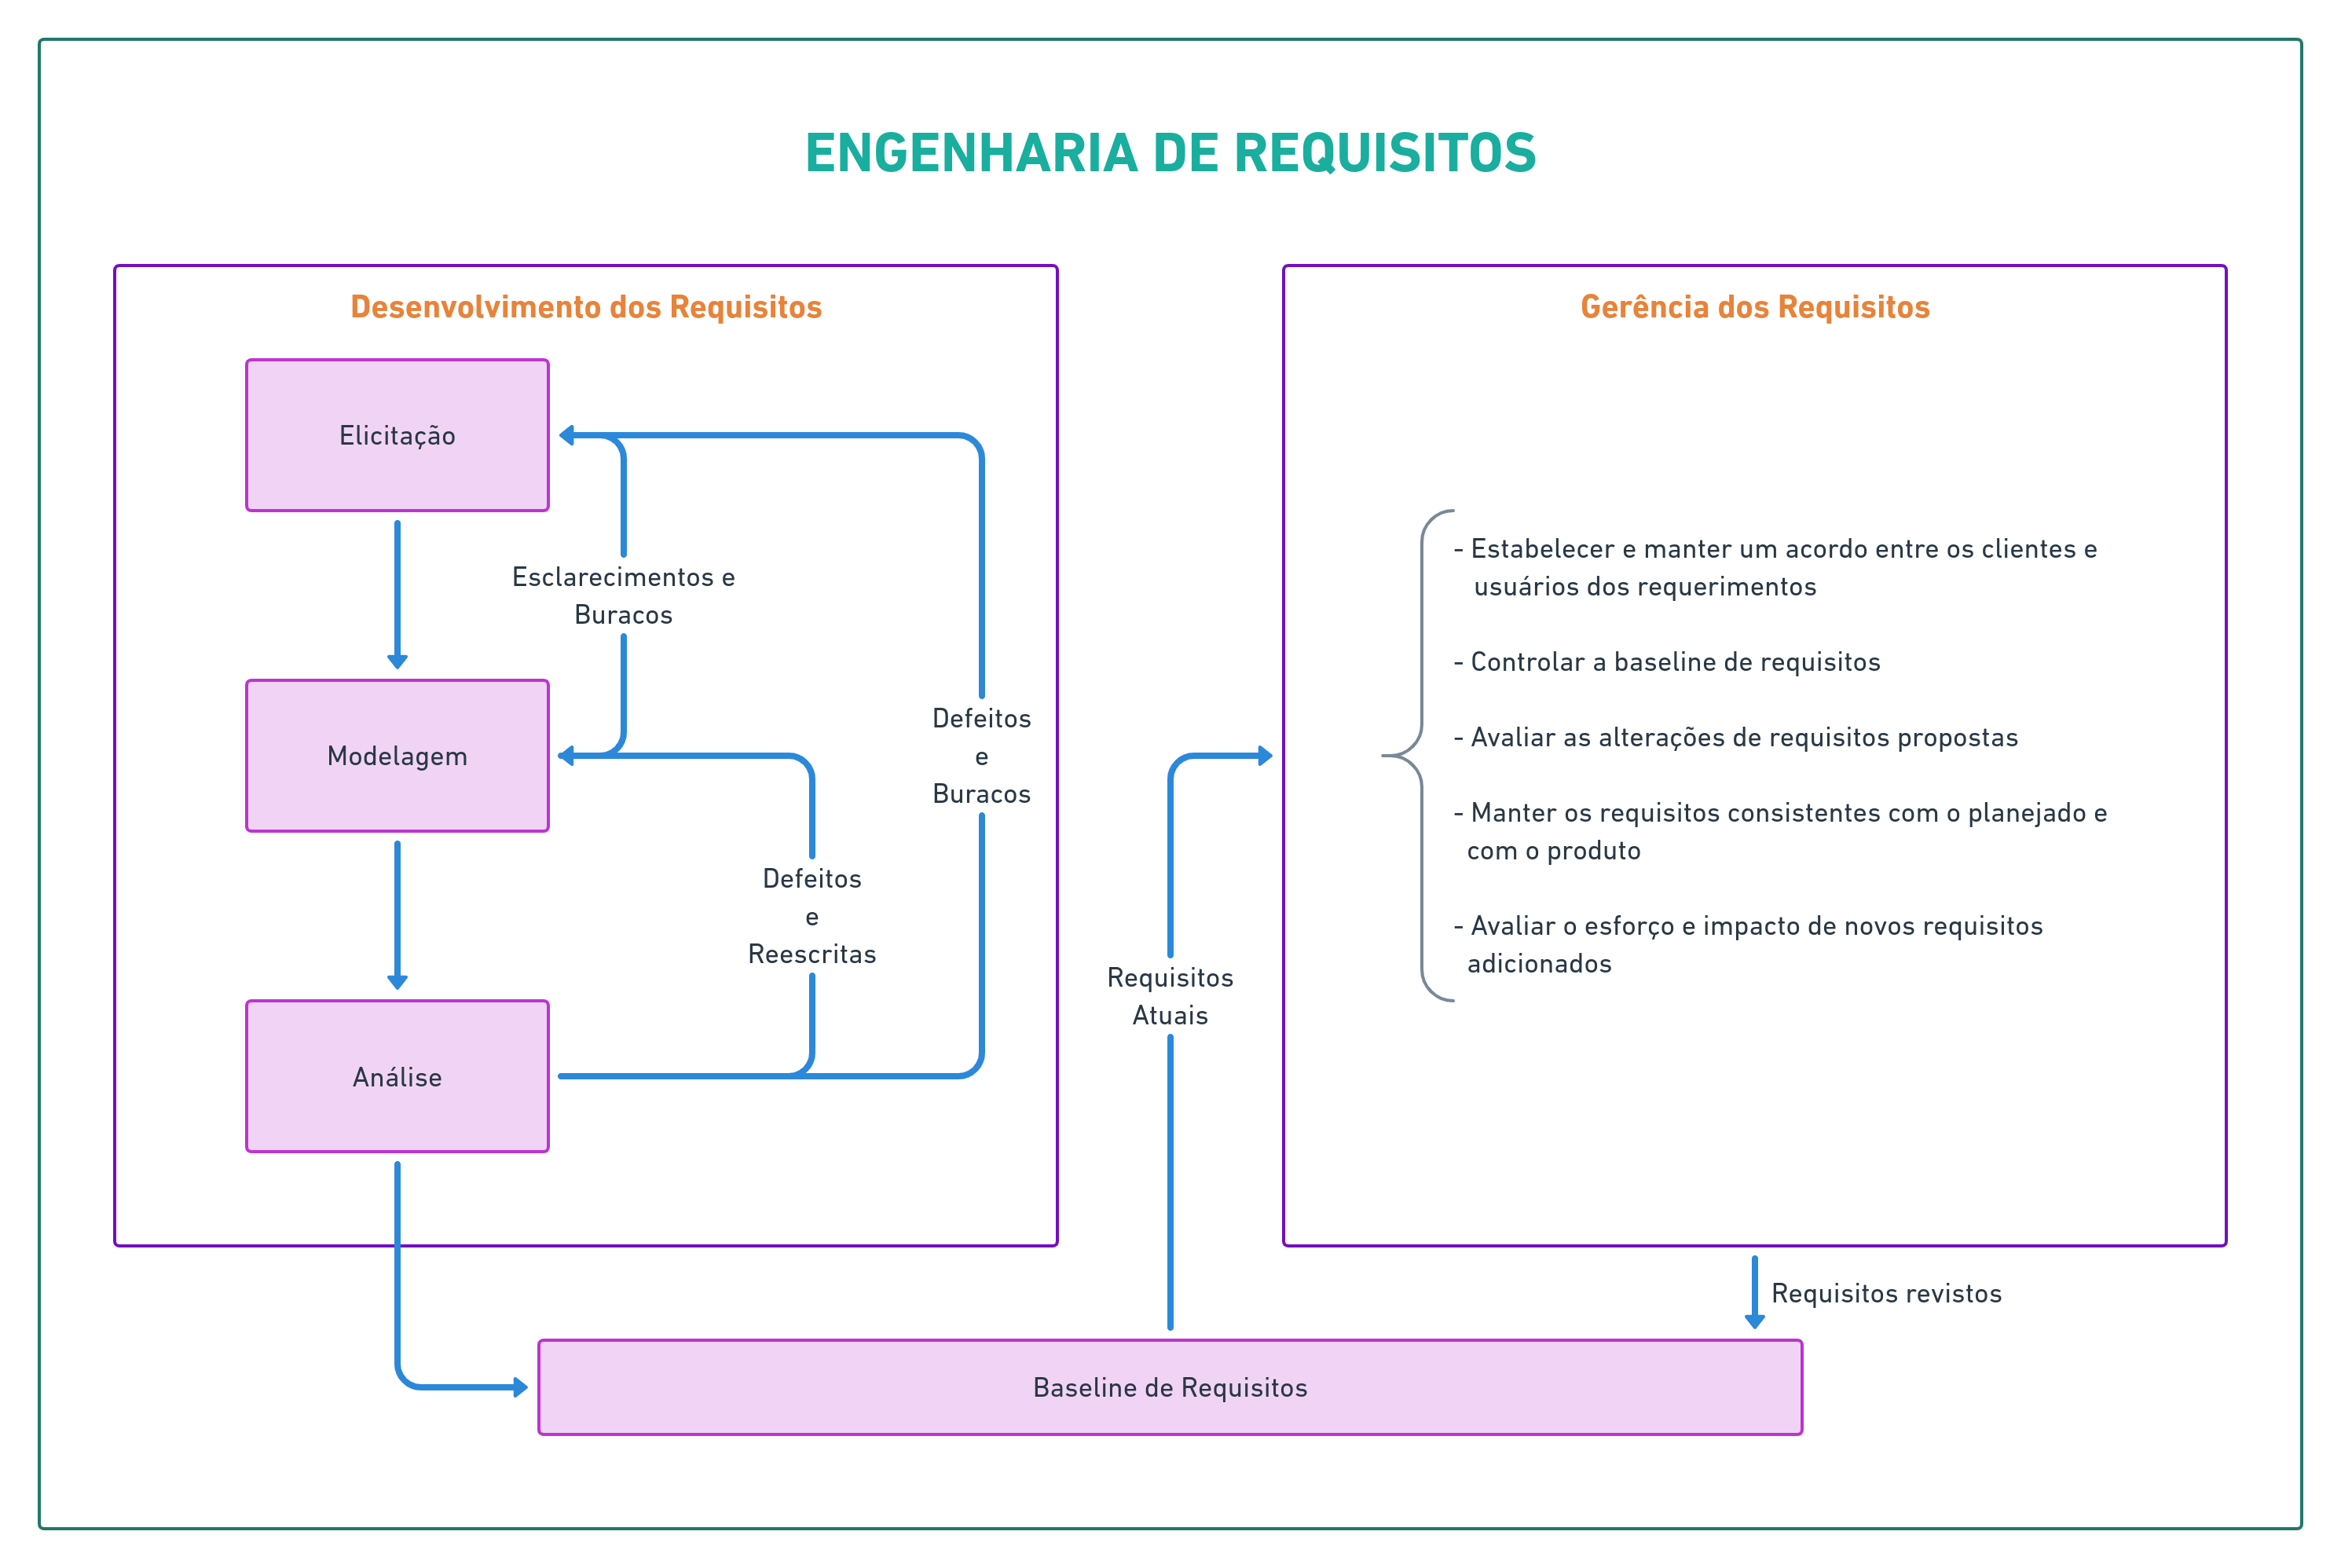
\includegraphics[scale=0.15]{figuras/Embasamento/eng_req_fluxo.png}
            \legend{Fonte: Adaptação de \citeauthoronline{westfall_5w2h}, \citeyear{westfall_5w2h}}
        \end{center}
    \end{figure}
    
\end{itemize}

Como descrito anteriormente, a Engenharia de Requisitos é uma área essencial na construção de um produto de \textit{software}. Existem vários processos e várias técnicas utilizadas para que o produto final seja desenvolvido com qualidade, evitando retrabalhos no futuro. Alguns processos e técnicas utilizados na Engenharia de Requisitos serão tratados nas próximas seções.

\section{Rastreabilidade}

\label{sec:rastreabilidade}

\subsection{Pré-rastreabilidade}

\label{sec:pre-rastreabilidade}

A Pré-rastreabilidade preocupa-se, objetivamente, em rastrear um requisito até a sua origem (\textit{Backward-From}), ou da origem até o requisito (\textit{Forward-To}). De forma exemplificada, quando um requisito é alterado, usa-se a pré-rastreabilidade para investigar as informações utilizadas para obtê-lo, ou seja, para delinear a pessoa interessada, quais técnicas ou quais documentos o requisito foi extraído, dentre outros \cite{pinheiro2004requirements}. Pode-se ter o interesse ainda de rastrear da origem até o requisito. O importante é ter em mente que a pré-rastreabilidade está compreendida entre Origem-\textit{Baseline} de Requisitos (sentido avante) ou entre \textit{Baseline} de Requisitos-Origem (sentido reverso). Não é escopo de atuação da pré-rastreabilidade considerar rastros da \textit{Baseline} de Requisitos para outros níveis de abstração mais baixos, tais como Arquitetura e Código.

\subsubsection{5W2H}

\label{sec:5w2h}

5W2H é um acrônimo em inglês que representa as principais perguntas que devem ser feitas e respondidas para investigar e relatar um fato ou situação: \textit{Who}, \textit{What}, \textit{Where}, \textit{When}, \textit{Why}, \textit{How} e \textit{How Much}. O 5W2H é uma ferramenta empregada no planejamento estratégico de empresas, análise de negócios, elaboração de planos de negócios e outras áreas de gestão. Tem o objetivo de descrever um plano de ação com as atividades que precisam ser desenvolvidas com o máximo de clareza possível. Essa ferramenta baseia-se na elaboração de um artefato formado por sete perguntas: O quê? Por quê? Quem? Onde? Quando? Como? Quanto custa? \cite{rabuskeuso}. Seguem as perguntas, as quais estão apresentadas em português. Entretanto, em inglês, cabe ressaltar, fica mais compreensível o nome atribuído ao \textit{Framework} Conceitual 5W2H, com: \textit{What}, \textit{Why}, \textit{Who}, \textit{Where}, \textit{When}, \textit{How}, e \textit{How Much}, respectivamente.

\begin{itemize}
    \item O quê?: que ação será executada;
    \item Por quê?: porque a ação será executada;
    \item Quem?: quem irá participar da ação;
    \item Onde?: onde será executada a ação;
    \item Quando?: quando a ação será executada;
    \item Como?: como a ação será executada, e
    \item Quanto custa?: quanto custa para executar a ação.
\end{itemize}

A Tabela \ref{quadro:5w2h_ex} ilustra um exemplo de 5W2H, realizado para a aplicação \textit{iGado} (\citeonline{quadro_igado}), que tem o objetivo de facilitar o gerenciamento rural de forma que o proprietário possa ter um controle sobre os dados dos seus bovinos. Ressalta-se que como esse artefato permite rastros para vários aspectos relevantes do \textit{software}, incluindo \textit{Stakeholders}, fontes, funcionalidades, dentre outras, há pré-rastreabilidade anotada.

\begin{quadro}
\caption{5W2H do Aplicativo iGado}
\label{quadro:5w2h_ex}
\centering
\begin{tabular}{C{0.07\textheight}|p{0.55\textheight}}
    \hline
    O quê? & Um aplicativo para o gerenciamento e gestão da pecuária.\\ \hline
    Por quê? & Atualmente, no mercado, tem-se uma escassez de aplicativos para a gestão da pecuária. Além disso, muitos proprietários de fazenda ainda utilizam ferramentas arcaicas, como papel e caneta, para o gerenciamento da fazenda e, principalmente, da pecuária. \\ \hline
    Quem? & Alunos de Engenharia de \textit{Software} da Universidade de Brasília do Campus FGA-Gama que estão cursando a disciplina Arquitetura e Desenho de \textit{Software}. Haverá a participação de 2 \textit{stakeholders}, que irão auxiliar no processo de desenvolvimento do \textit{software}. \\ \hline
    Onde? & O projeto será realizado remotamente devido à pandemia. O aplicativo será disponibilizado para dispositivos mobile - \textit{iOS} e \textit{Android} \\ \hline
    Quando? & O usuário poderá acessar o aplicativo em qualquer momento. Quando houver a necessidade de anotar informações, visualizar dados e gerar relatórios. \\ \hline
    Como? & Por meio do desenvolvimento de um aplicativo mobile — iOS e Android, para facilitar o controle da gestão rural e permitir a geração de relatórios. O usuário poderá cadastrar as informações dos bovinos no aplicativo, além de ter uma janela para que o usuário gere os relatórios especificados por ele. \\ \hline
     Quanto Custa? & ~ R\$ 226.551,64 \\ \hline
\end{tabular}
\legend{Fonte: Autores, 2022.}
\end{quadro}

\subsubsection{\textit{Rich Picture}}

\label{sec:rich_picture}

\textit{Rich Picture} é uma ilustração que visa identificar as partes interessadas(\textit{stakeholders}), suas preocupações e partes subjacentes. É uma ferramenta para registrar e raciocinar sobre os aspectos do contexto de trabalho e como eles afetam o produto  \cite{10.1145/274430.274434}. Além disso, ela se baseia em rascunhar desenhos e usar textos curtos e objetivos para expressar um momento, um desejo, uma atividade, dentre outras necessidades. A Figura \ref{fig:rich_picture}, desenvolvido para a aplicação \textit{Pax} (\citeonline{pax_app}), ilustra um exemplo de \textit{Rich Picture} no contexto de uma aplicação cujo foco é conectar prestadores de serviços aos seus possíveis clientes. Cabe ressaltar que esse artefato, por revelar fontes de informação (ex. Leis e Termos de Uso); \textit{Stakeholders} (ex. Prestador de Serviços e Usuário), fluxos de atividades (ex. Prestador de Serviços aceita Termos de Uso), dentre outras informações do Universo de Informações \cite{leite2007livro}, permite conferir pré-rastreabilidade.

\begin{figure}[htb]
    \begin{center}
        \caption{Rich Picture do Aplicativo PAX}
        \label{fig:rich_picture}
        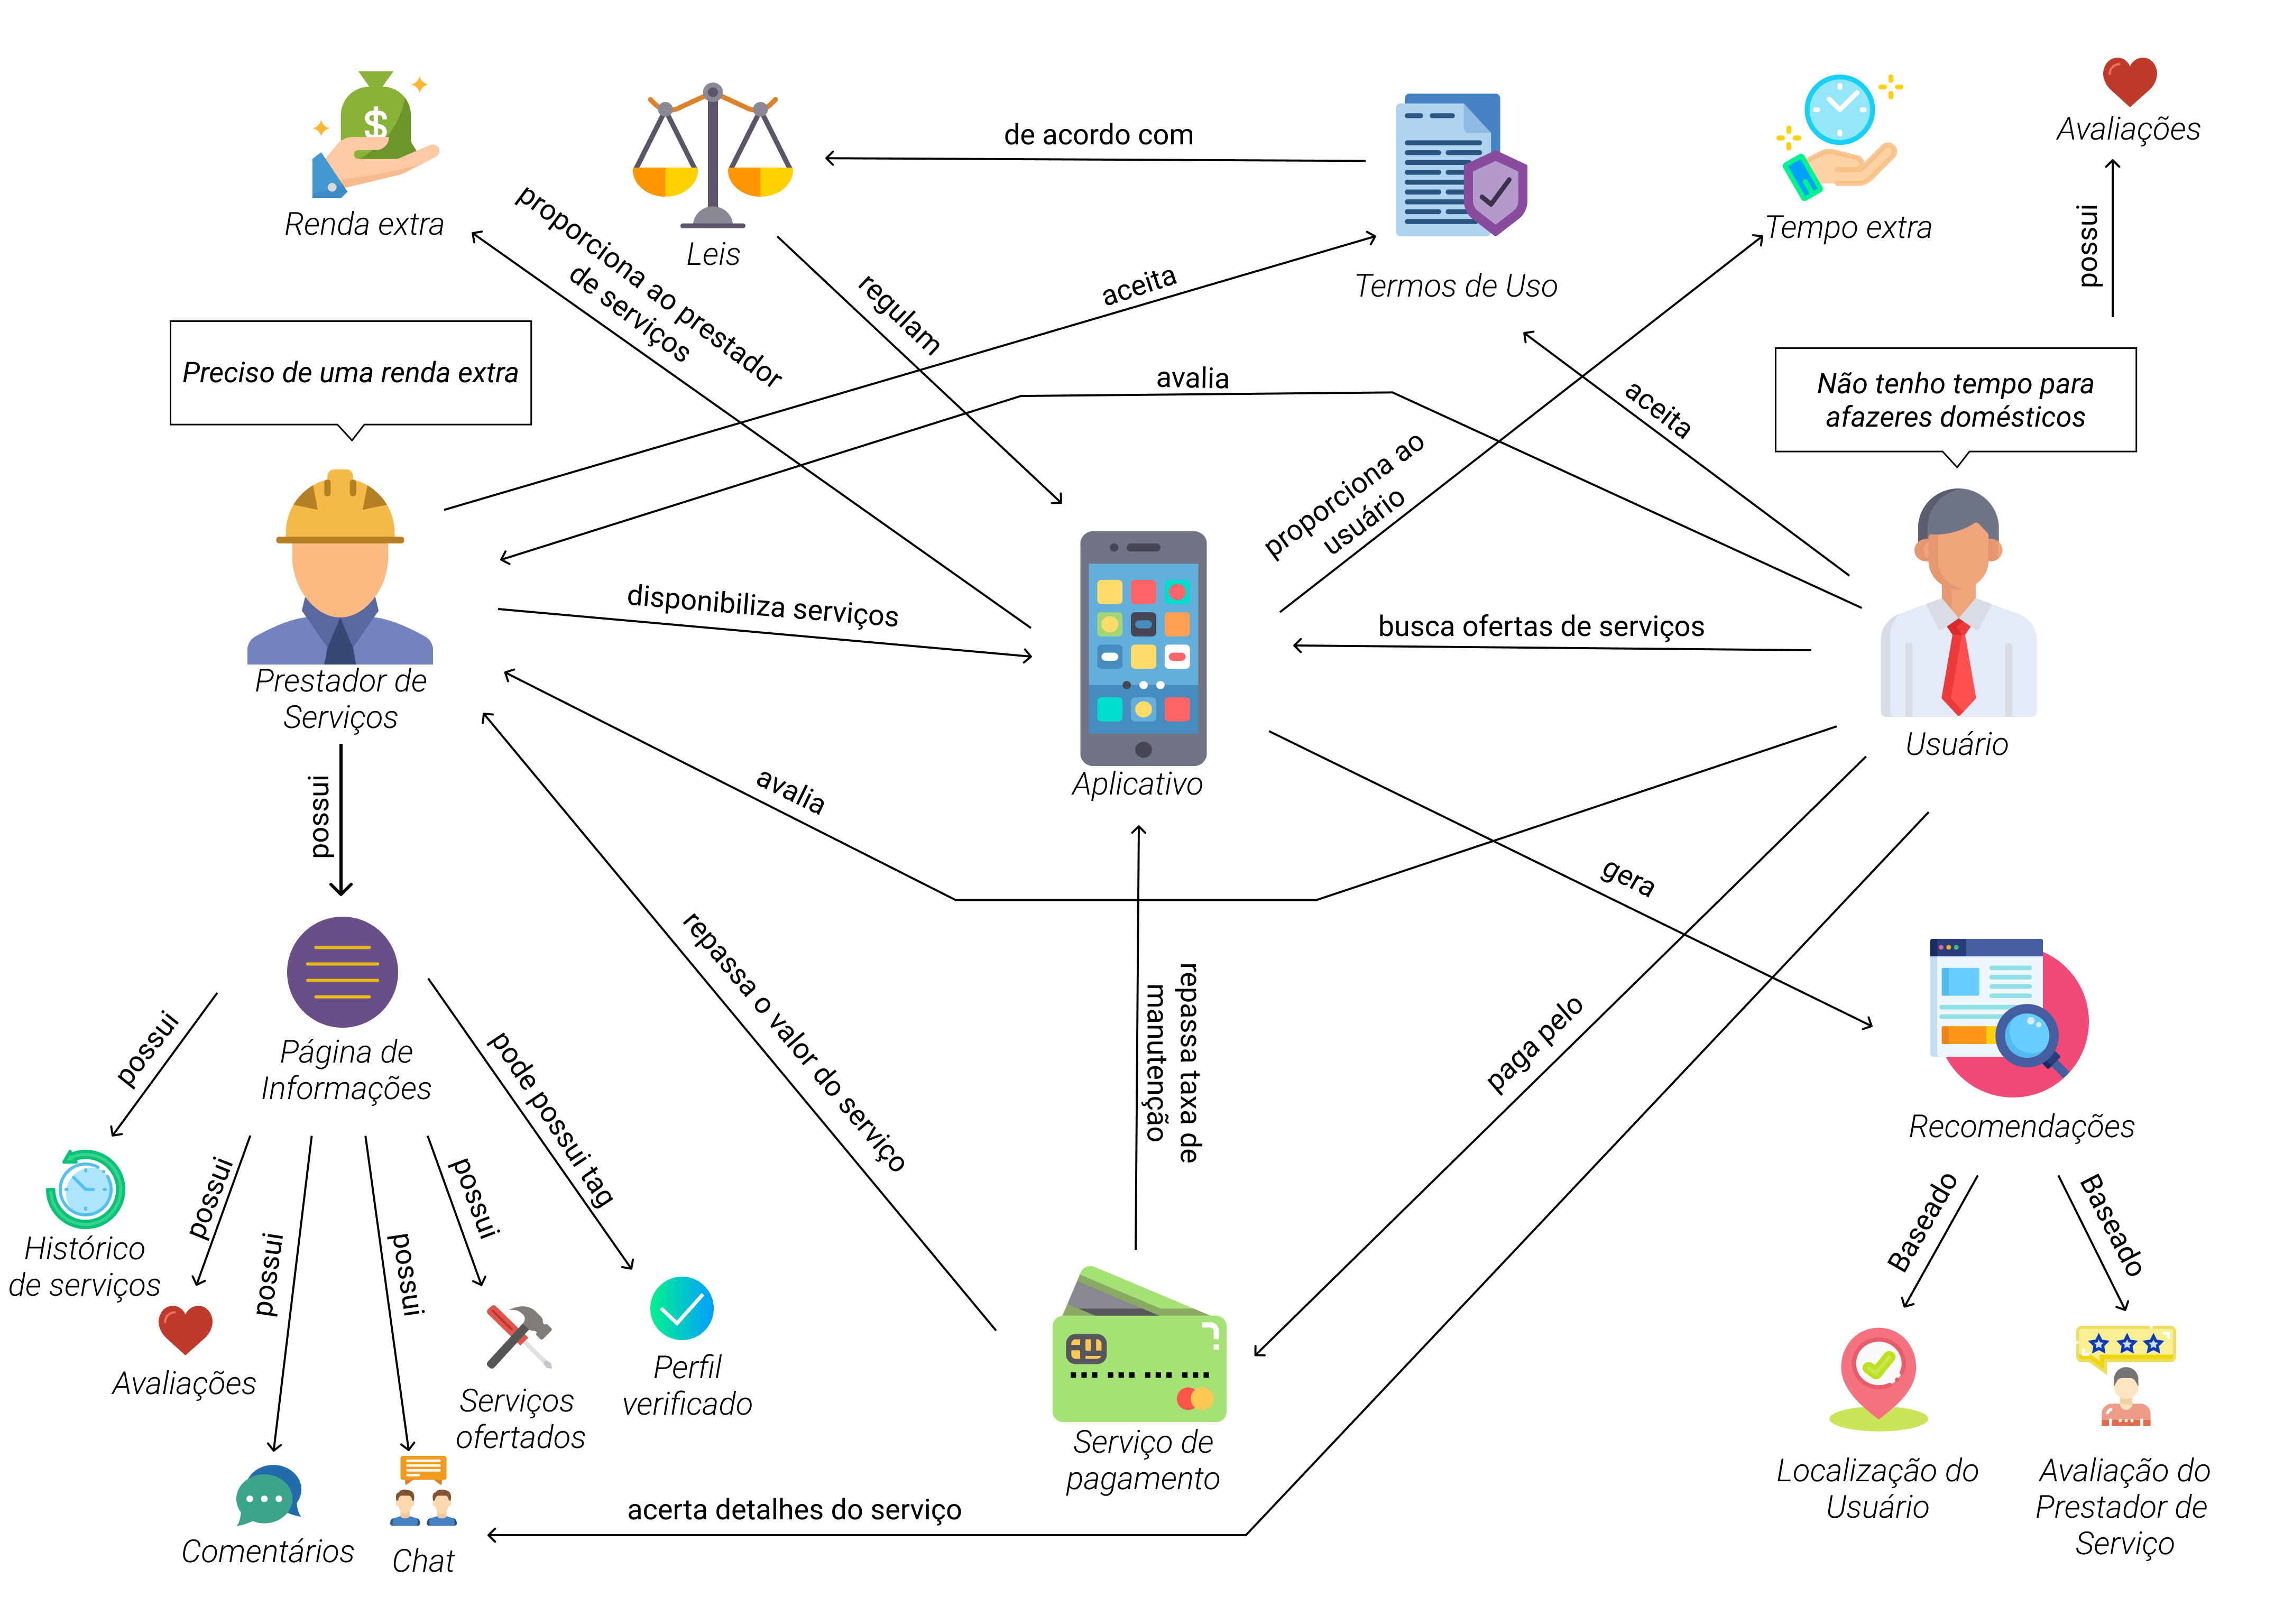
\includegraphics[scale=0.31]{figuras/Embasamento/rp_geral_v3.png}
        \legend{Fonte: Autores, 2022.}
    \end{center}
\end{figure}

\subsection{Pós-rastreabilidade}

\label{sec:pos-rastreabilidade}

A Pós-rastreabilidade consiste em rastrear um requisito para a implementação de um projeto. Exemplificadamente, quando um requisito é alterado, usa-se a pós-rastreabilidade para investigar o impacto desta mudança, no nível de implementação. Portanto, \textit{Forward-from}, consistindo em ligar o requisito do sistema ao código, e mantendo o conhecimento de onde o requisito está implementado, e qual foi o caminho percorrido por ele, da \textit{baseline} de requisitos, passando pelas etapas de desenho e arquitetura, teste e código. Há ainda, a possibilidade de realizar o sentido reverso, \textit{Backward-to}. Neste caso, e dentro do contexto de Pós-rastreabilidade, permite-se ligar o código aos requisitos do sistema \cite{pinheiro2004requirements}.

\section {Elicitação}

\label{sec:elicitacao}

A Elicitação de Requisitos é o processo relacionado às atividades que permitem a compreensão de metas, objetivos e motivos para a construção de um novo sistema de \textit{software}, e a identificação dos requisitos associados às partes interessadas, no intuito de compreender o sistema a ser desenvolvido \cite{elliott2012software}.

Além disso, as informações coletadas durante a elicitação de requisitos, geralmente, precisam ser modeladas e analisadas (verificadas e validadas), antes do início da implementação do sistema \cite{nuseibeh2000requirements}.

\subsection{\textit{Brainstorming}}

\label{sec:brainstorming}

O \textit{Brainstorming} ou “Tempestade de Ideias”, por ser uma técnica de grupo, tem o objetivo de coletar o maior número de ideias acerca de um determinado tema ou questão. É utilizada, geralmente, na fase de planejamento de um projeto. Propõe que um grupo de pessoas se reúnam de modo a colaborar para uma “tempestade de ideias”, onde cada ideia é conferida e acrescentada, para gerar um longo processo de sugestões e discussões. Vale ressaltar que nenhuma ideia, inicialmente, é criticada ou julgada \cite{mazzotti2012exploraccao}.

O \textit{Brainstorming} é usado para gerar novas ideias, deixando a mente livre para aceitar todas as ideias sugeridas e, assim, permitir a liberdade para a criatividade \cite{batista2003taxonomia}. Uma dificuldade é documentar um \textit{Brainstorming}. Entretanto, pode-se usar desde gravações em vídeos e áudios, e até mesmo Mapas Mentais e outros modelos que permitem rápidas anotações.

A Figura \ref{fig:mind_map}, desenvolvida para a aplicação \textit{iGado} (\citeonline{quadro_igado}), mostra um \textit{Mapa Mental}, especificado a partir de um debate no contexto de elicitação de um \textit{software} no domínio de uma aplicação \textit{mobile}, que visa facilitar o gerenciamento rural de proprietários de fazendas, em que a equipe usava a técnica de \textit{Brainstorming}.

\begin{figure}[H]
    \begin{center}
        \caption{Mapa Mental do Aplicativo iGado}
        \label{fig:mind_map}
        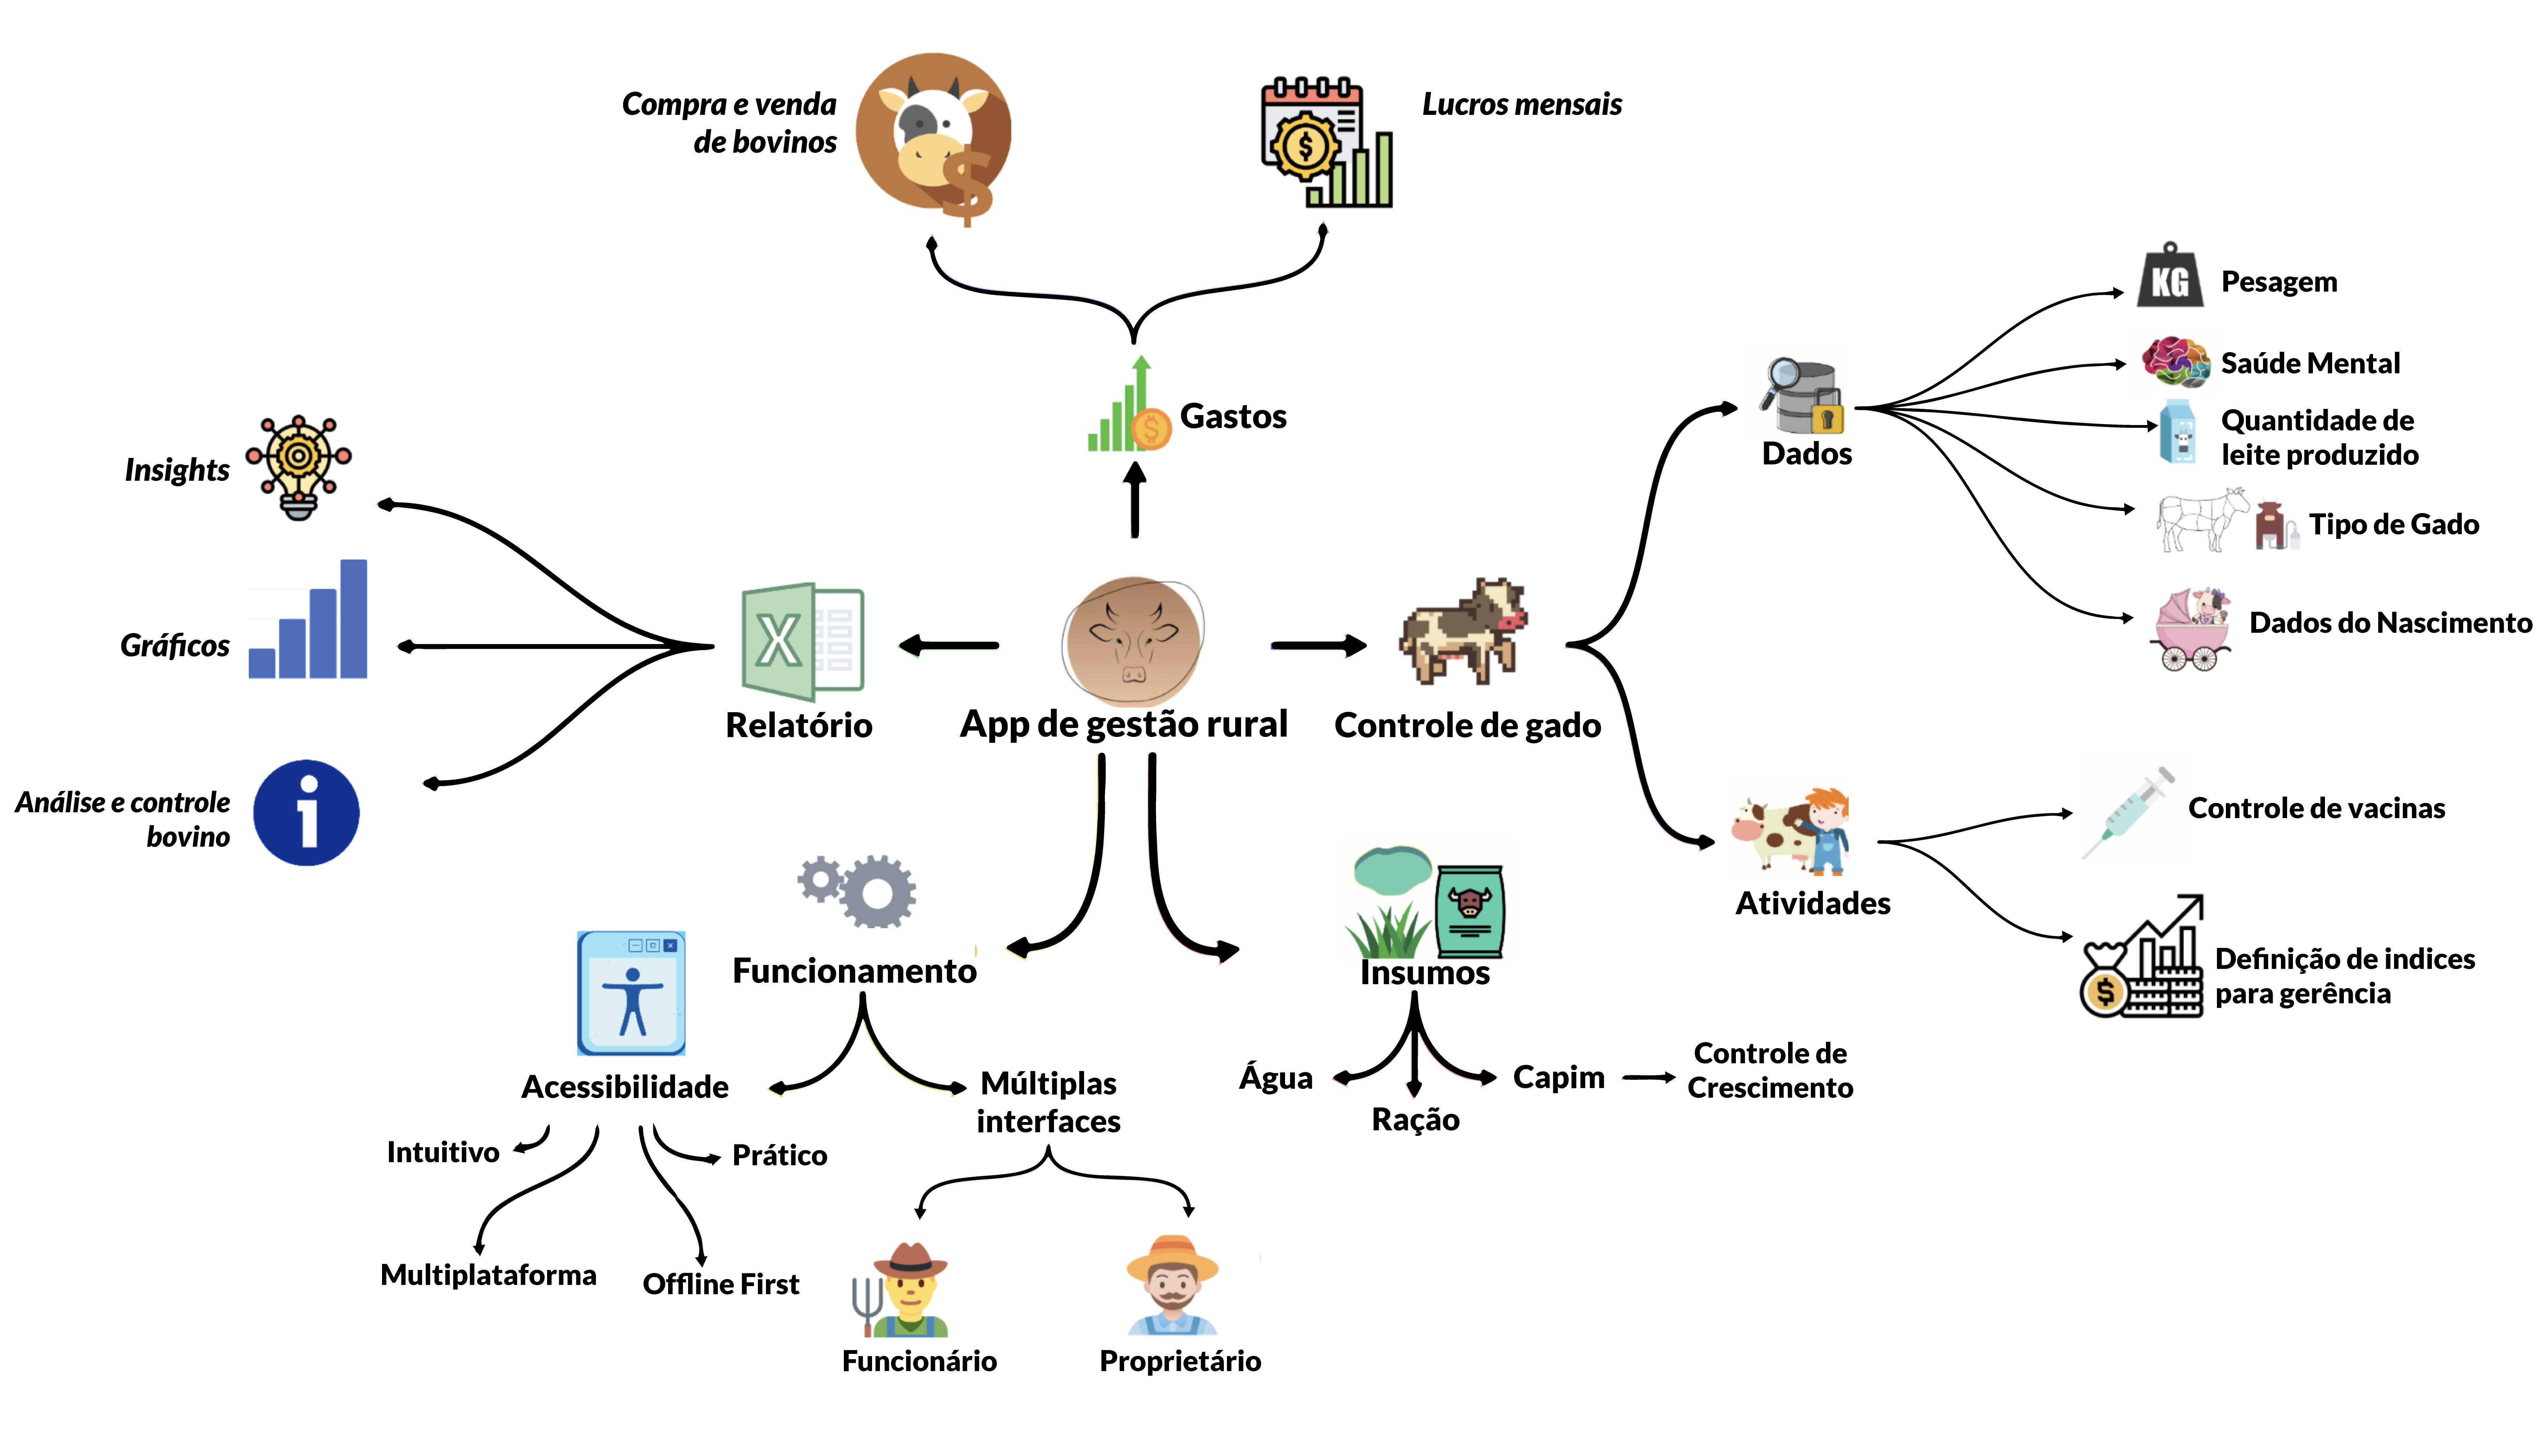
\includegraphics[scale=0.25]{figuras/Embasamento/MindMap_v2.png}
        \legend{Fonte: Autores, 2022.}
    \end{center}
\end{figure}

\subsection{Questionário}

\label{sec:questionario}

O Questionário é uma técnica de coleta de informações que permite aos envolvidos no projeto estudar atitudes, crenças, comportamentos e características do público alvo que podem ser afetados pelo sistema atual e pelo sistema proposto \cite{kendall1992systems}. Deve ser realizada com muita cautela. A elaboração das perguntas, que vão constituir o questionário, é um processo engenhoso, complexo e delicado. Um questionário mal elaborado pode, facilmente, levar a conclusões errôneas, que acabam sendo prejudiciais para o projeto que está sendo desenvolvido \cite{bastosjunior}.

De acordo com \citeonline{segundo2017custom}, um questionário deve ser elaborado tendo em mente alguns aspectos-chave, dentre eles: 

\begin{enumerate}
    \item Coleta de informações sobre o perfil dos participantes; 
    \item A informação que se quer descobrir, onde devem ser considerada, primeiramente, uma mensagem  introdutória, direcionando o participante sobre o questionamento, seja essa de múltipla escolha ou mais discursiva, e
    \item Análise dos resultados obtidos, procurando apresentá-los usando gráficos, tabelas, e quadros bem claros e objetivos, com base, preferencialmente, em diferentes pontos de vista.
\end{enumerate}

\subsection{Protótipo de Baixa Fidelidade}

\label{sec:prototipo-def}

Um Protótipo, segundo \citeonline{Sommerville10}, “é uma versão inicial de um sistema de \textit{software}, usado para demonstrar conceitos, experimentar opções de projeto e descobrir mais sobre o problema e suas possíveis soluções”. É muito significativo no processo de Engenharia de Requisitos pelo fato de ajudar na elicitação dos requisitos de \textit{software}, e para estudar soluções específicas do \textit{software}.

\subsection{\textit{Storytelling}}

\label{sec:storytelling}

\textit{Storytelling}, ou simplesmente História, é uma técnica que busca, por meio da análise da descrição de algum processo ou tarefa realizado em algum contexto, extrair \textit{features} do sistema. Vale ressaltar que não existe um formato ou estrutura pré-definida, mas há descrições de altos níveis de uso do sistema. As \textit{Storytellings} são muito usadas, visando conferir um panorama do sistema  \cite{Sommerville10}.

O próprio cérebro humano, segundo estudos, é mais propenso ao aprendizado proveniente de histórias. Por retratarem a experiência de quem conta, sendo essa validada pelo próprio orador, as narrativas proporcionam um retrato realista e lógico de algo vivido por seu interlocutor. Isso proporciona um entendimento com uma carga de sentimentos e fatos que podem ser usados para a extração de requisitos mais ricos  \cite{storytelling}.

\subsection{Entrevista}

\label{sec:entrevista}

Entrevista é uma das técnicas mais utilizadas por possuir uma comunicação mais natural entre as pessoas. As entrevistas são usadas para a obtenção de conhecimento sobre um determinado tema/domínio, por perguntas feitas aos usuários especialistas, além de trazer muitas informações aos desenvolvedores do projeto \cite{batista2003taxonomia}. De acordo com \citeonline{Sommerville10}, elas podem ser de dois tipos:
\begin{itemize}
    \item Fechadas: seguem um conjunto de perguntas pré-definidas, e
    \item Abertas: não se tem uma agenda pré-definida.
\end{itemize}
Na prática, geralmente, as entrevistas são híbridas, orientando-se por ambos os tipos.

\subsection{Análise de Protocolo}

\label{sec:analise-protocolo}

A Análise de Protocolo consiste em pedir a uma pessoa para que ela se envolva em uma tarefa, e fale em voz alta o seu processo de pensamento. Sendo assim, têm-se insumos para ocorrer a extração de possíveis requisitos do sistema \cite{goguen1993techniques}. Usuários alegam que essa categoria de linguagem pode ser considerada uma “verbalização direta do processo cognitivo específico”. Vale ressaltar que a Análise de Protocolo está sujeita a problemas de interpretações pelos analistas \cite{belgamo2000estudo}.

\section {Modelagem}

\label{sec:modelagem}

Esta parte do processo da Engenharia de Requisitos consiste em estruturar os requisitos levantados no período da elicitação (Seção \ref{sec:elicitacao}) de forma sistemática. De acordo com \citeonline{Sommerville10}, os requisitos “devem ser claros, inequívocos, fáceis de entender, completos e consistentes”.

Vale mencionar que os documentos gerados, nesta fase, devem ser de fácil entendimento para os \textit{stakeholders} do projeto, sem existirem detalhes técnicos de implementação ou arquitetura do sistema \cite{Sommerville10}.

\subsection{\textit{Backlog}}

\label{sec:backlog}

O \textit{Backlog} do Produto é um artefato essencial na Engenharia de Requisitos, na metodologia ágil e no ciclo de desenvolvimento de um produto, pois os requisitos elicitados constam nele. Em uma definição mais concreta, o \textit{Backlog} é uma lista ordenada e emergente do que é necessário no produto (segundo os \textit{Stakeholders} consultados), ou seja, é um artefato que agrupa os requisitos \cite{carolipaulo2021}. As funcionalidades são descritas no \textit{Backlog}, sendo esse o que o cliente espera receber ao final do projeto.

Dentro desta construção, \citeauthoronline{carolipaulo2021} (\citeyear{carolipaulo2021}) delimita alguns conceitos usados para uma definição mais consistente dos requisitos, sendo elas:

\begin{enumerate}
    \item \label{tp:epico} \textbf{Épico}: é uma grande parte de trabalho que, geralmente, é dividida em tarefas menores, ou seja, histórias de usuário. Trata-se de um trabalho realizado em semanas ou meses;
    \item \label{tp:feature} \textit{\textbf{Feature}}: é uma funcionalidade que faz parte de um módulo, possuindo seus requisitos funcionais e suas regras de negócio. Trata-se de alguma ação ou interação do usuário com o produto, e
    \item \label{tp:us} \textbf{História de Usuário}: é uma função da \textit{feature}, e está associado a ela. Objetivamente, equivale aos requisitos funcionais de uma \textit{interface}. Além disso, trata-se de uma pequena parte da funcionalidade que faz sentido para os \textit{stakeholders}.
\end{enumerate}

Dessa forma, foi construído o \textit{backlog} da ferramenta proposta, podendo ser observado no Apêndice \ref{ap:backlog}.

\subsection{NFR}

\label{sec:nfr}

O NFR \textit{Framework} (\textit{Non-Functional Requirements}) é um artefato que visa tratar os requisitos não funcionais, expressando-os sistematicamente, e usando-os para guiar o processo de desenvolvimento do \textit{software}.

Segundo \citeonline{coutoproposta}, trata-se de uma abordagem que confere operacionalizações, considerando os requisitos não funcionais. Esses requisitos são especificados como metas a serem atingidas. Já as operacionalizações são vistas como ações concretas, que uma vez realizadas, colaboraram com o cumprimento das metas a serem atingidas.

Além disso, de acordo com \citeonline{chung2012non}, o “NFR \textit{Framework} usa os requisitos não funcionais como segurança, precisão, desempenho e custo para conduzir o processo geral de \textit{design}. O Framework visa colocar os requisitos não funcionais em primeiro lugar na mente do desenvolvedor”. A Figura \ref{fig:nfr_original} ilustra a mesma modelagem, em seu rigor de notação.

\begin{figure}[H]
    \begin{center}
        \caption{NFR com o Rigor da Notação}
        \label{fig:nfr_original}
        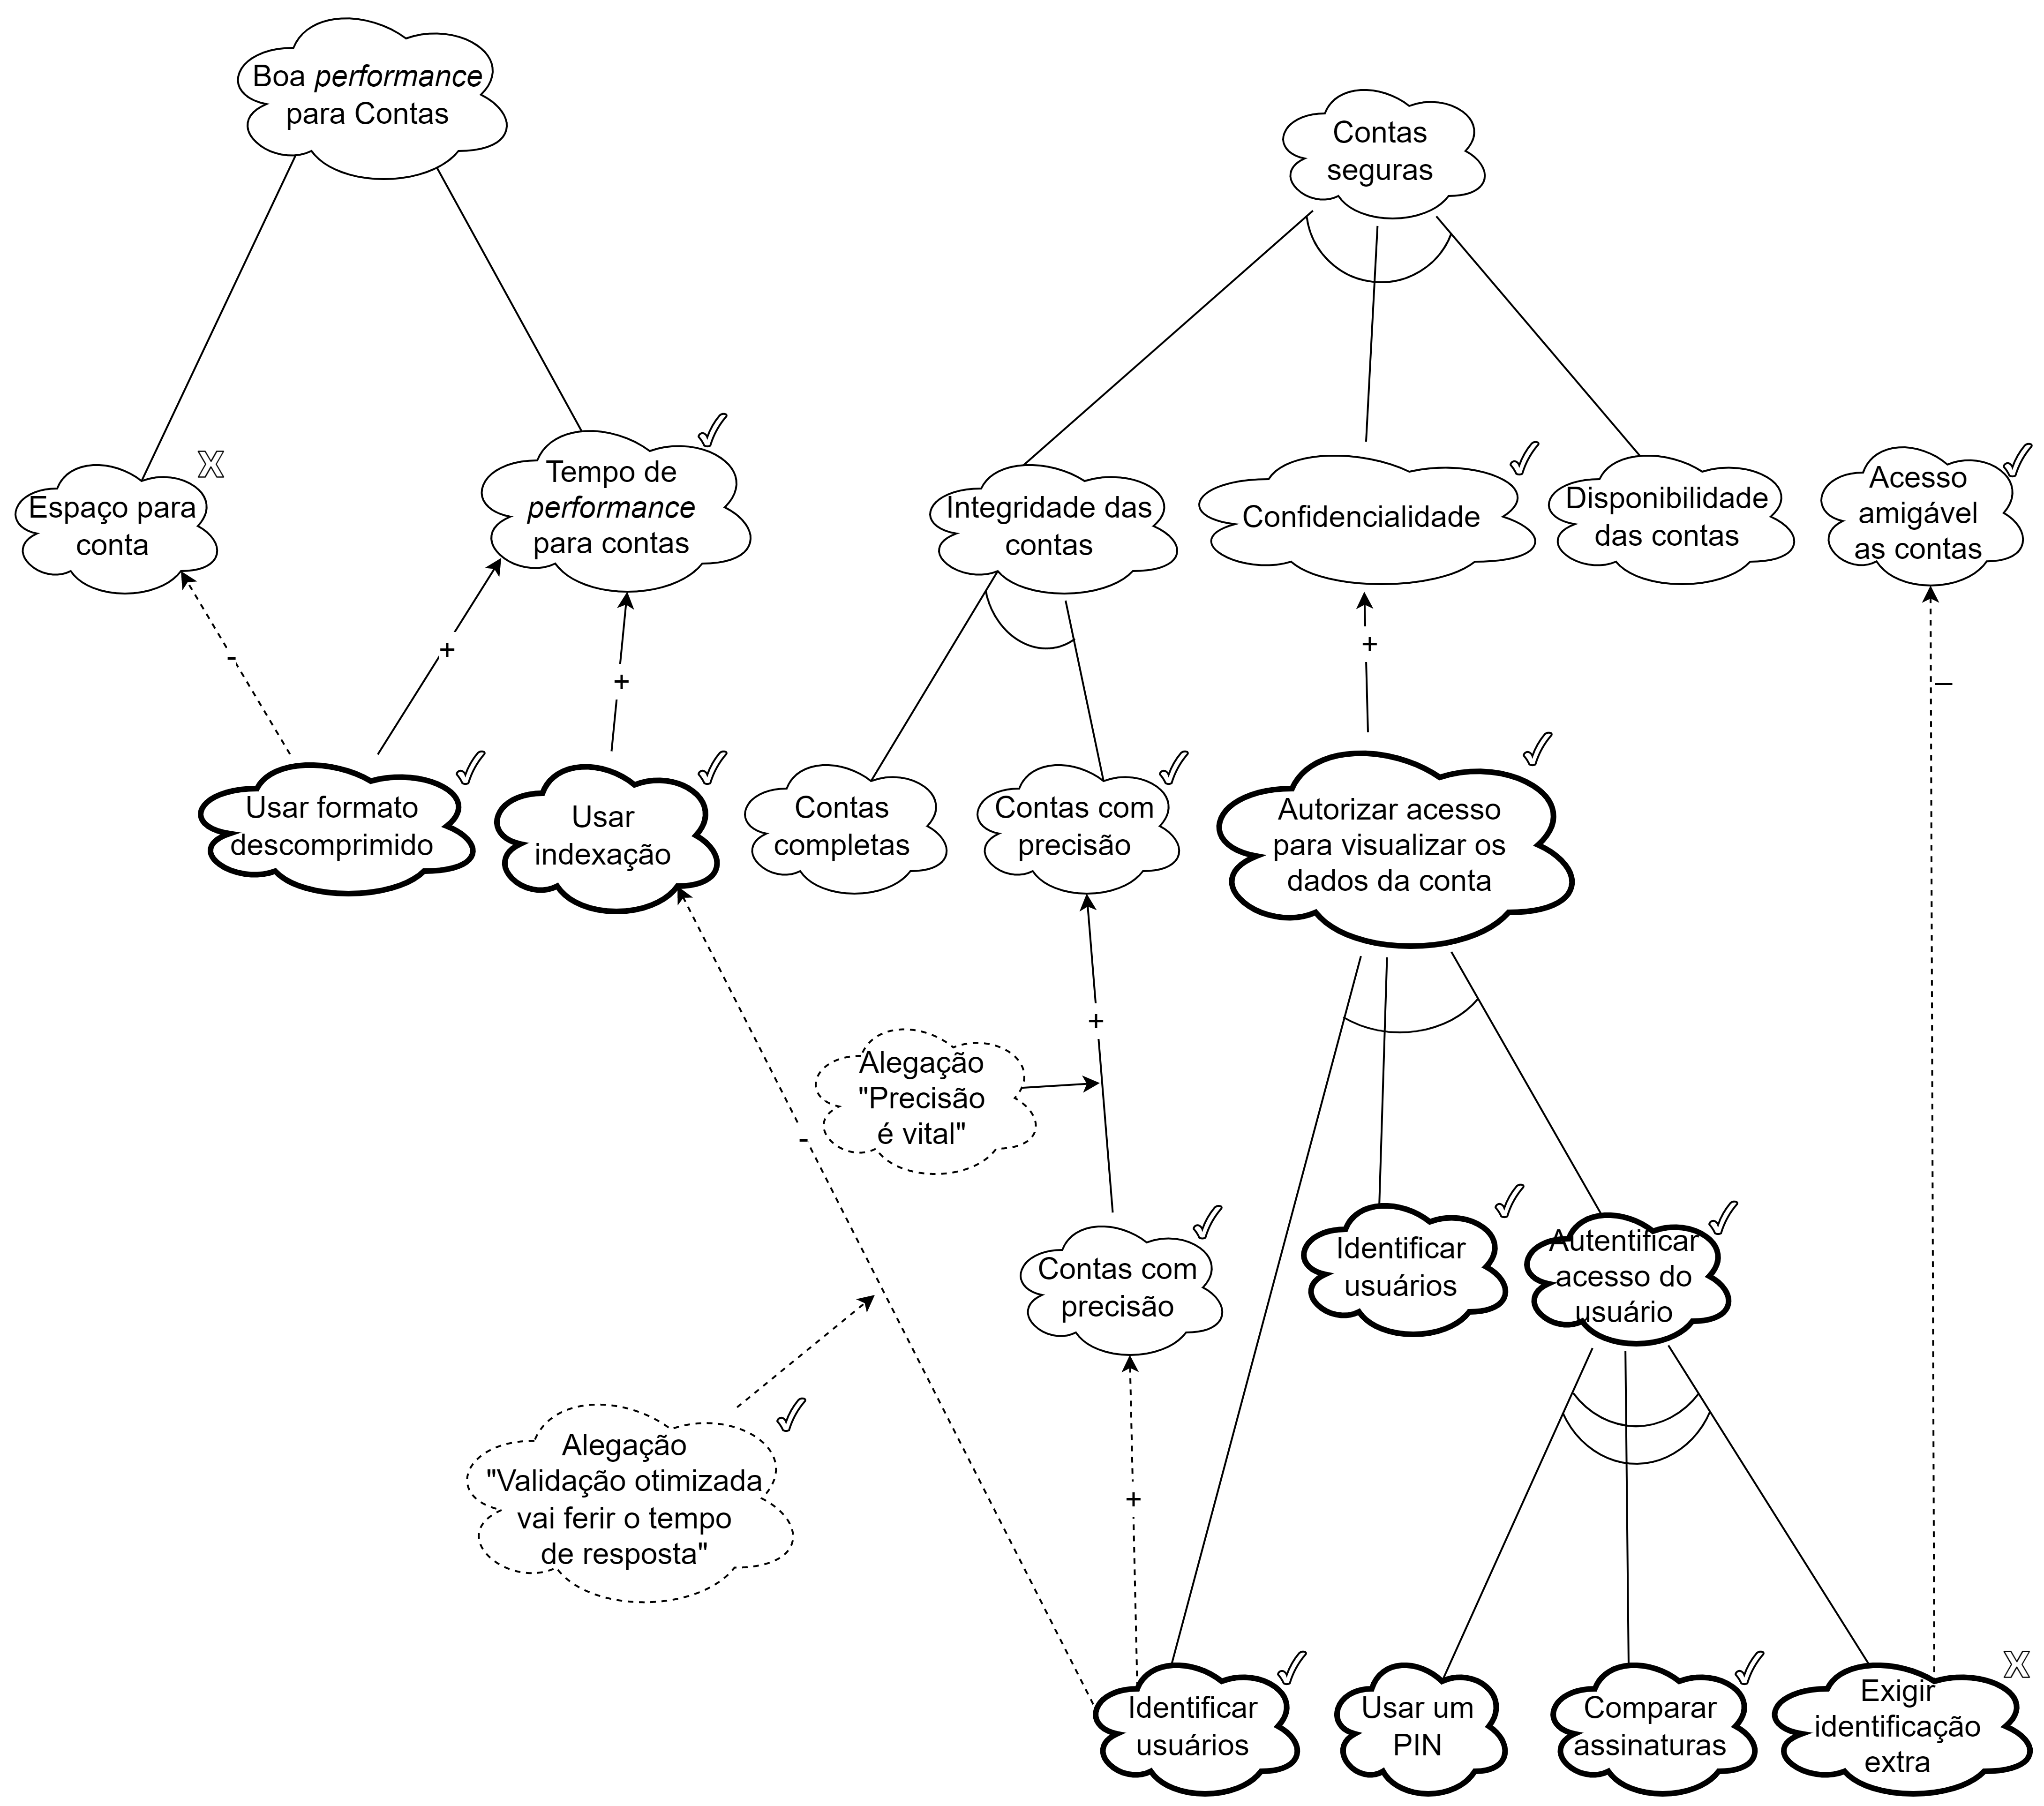
\includegraphics[scale=0.41]{figuras/Embasamento/nfr_rigor_v2.png}
        \legend{Fonte: Adaptado de \citeauthoronline{Ullah2011ASO}, \citeyear{Ullah2011ASO}.}
    \end{center}
\end{figure}


A intenção do presente trabalho foi usar os princípios desse modelo conceitual, visando um tratamento mais adequado dos requisitos não funcionais. Não foi utilizada a notação, em seu rigor. Entretanto, foi utilizado um processo guiado, orientando-se por esse modelo conceitual, e procurando facilitar o processo de modelagem dos requisitos não funcionais por parte dos usuários da ferramenta. Dessa forma, o NFR foi utilizado para definir os requisitos não funcionais de forma mais lapidada, ou seja, no seu segundo e/ou terceiro nível. Sendo assim, os requisitos não funcionais, na sua forma de operacionalização, foram modelados no \textit{House of Quality} (Seção \ref{sec:house_of_quality}).

A Figura \ref{fig:nfr_example} ilustra a adaptação usada na ferramenta, elaborada pelos autores, e orientada pelos princípios do NFR \textit{Framework}. O intuito é ser uma notação mais simples e compreensível aos usuários da ferramenta.

\begin{figure}[H]
    \begin{center}
        \caption{NFR Adaptado Proposto}
        \label{fig:nfr_example}
        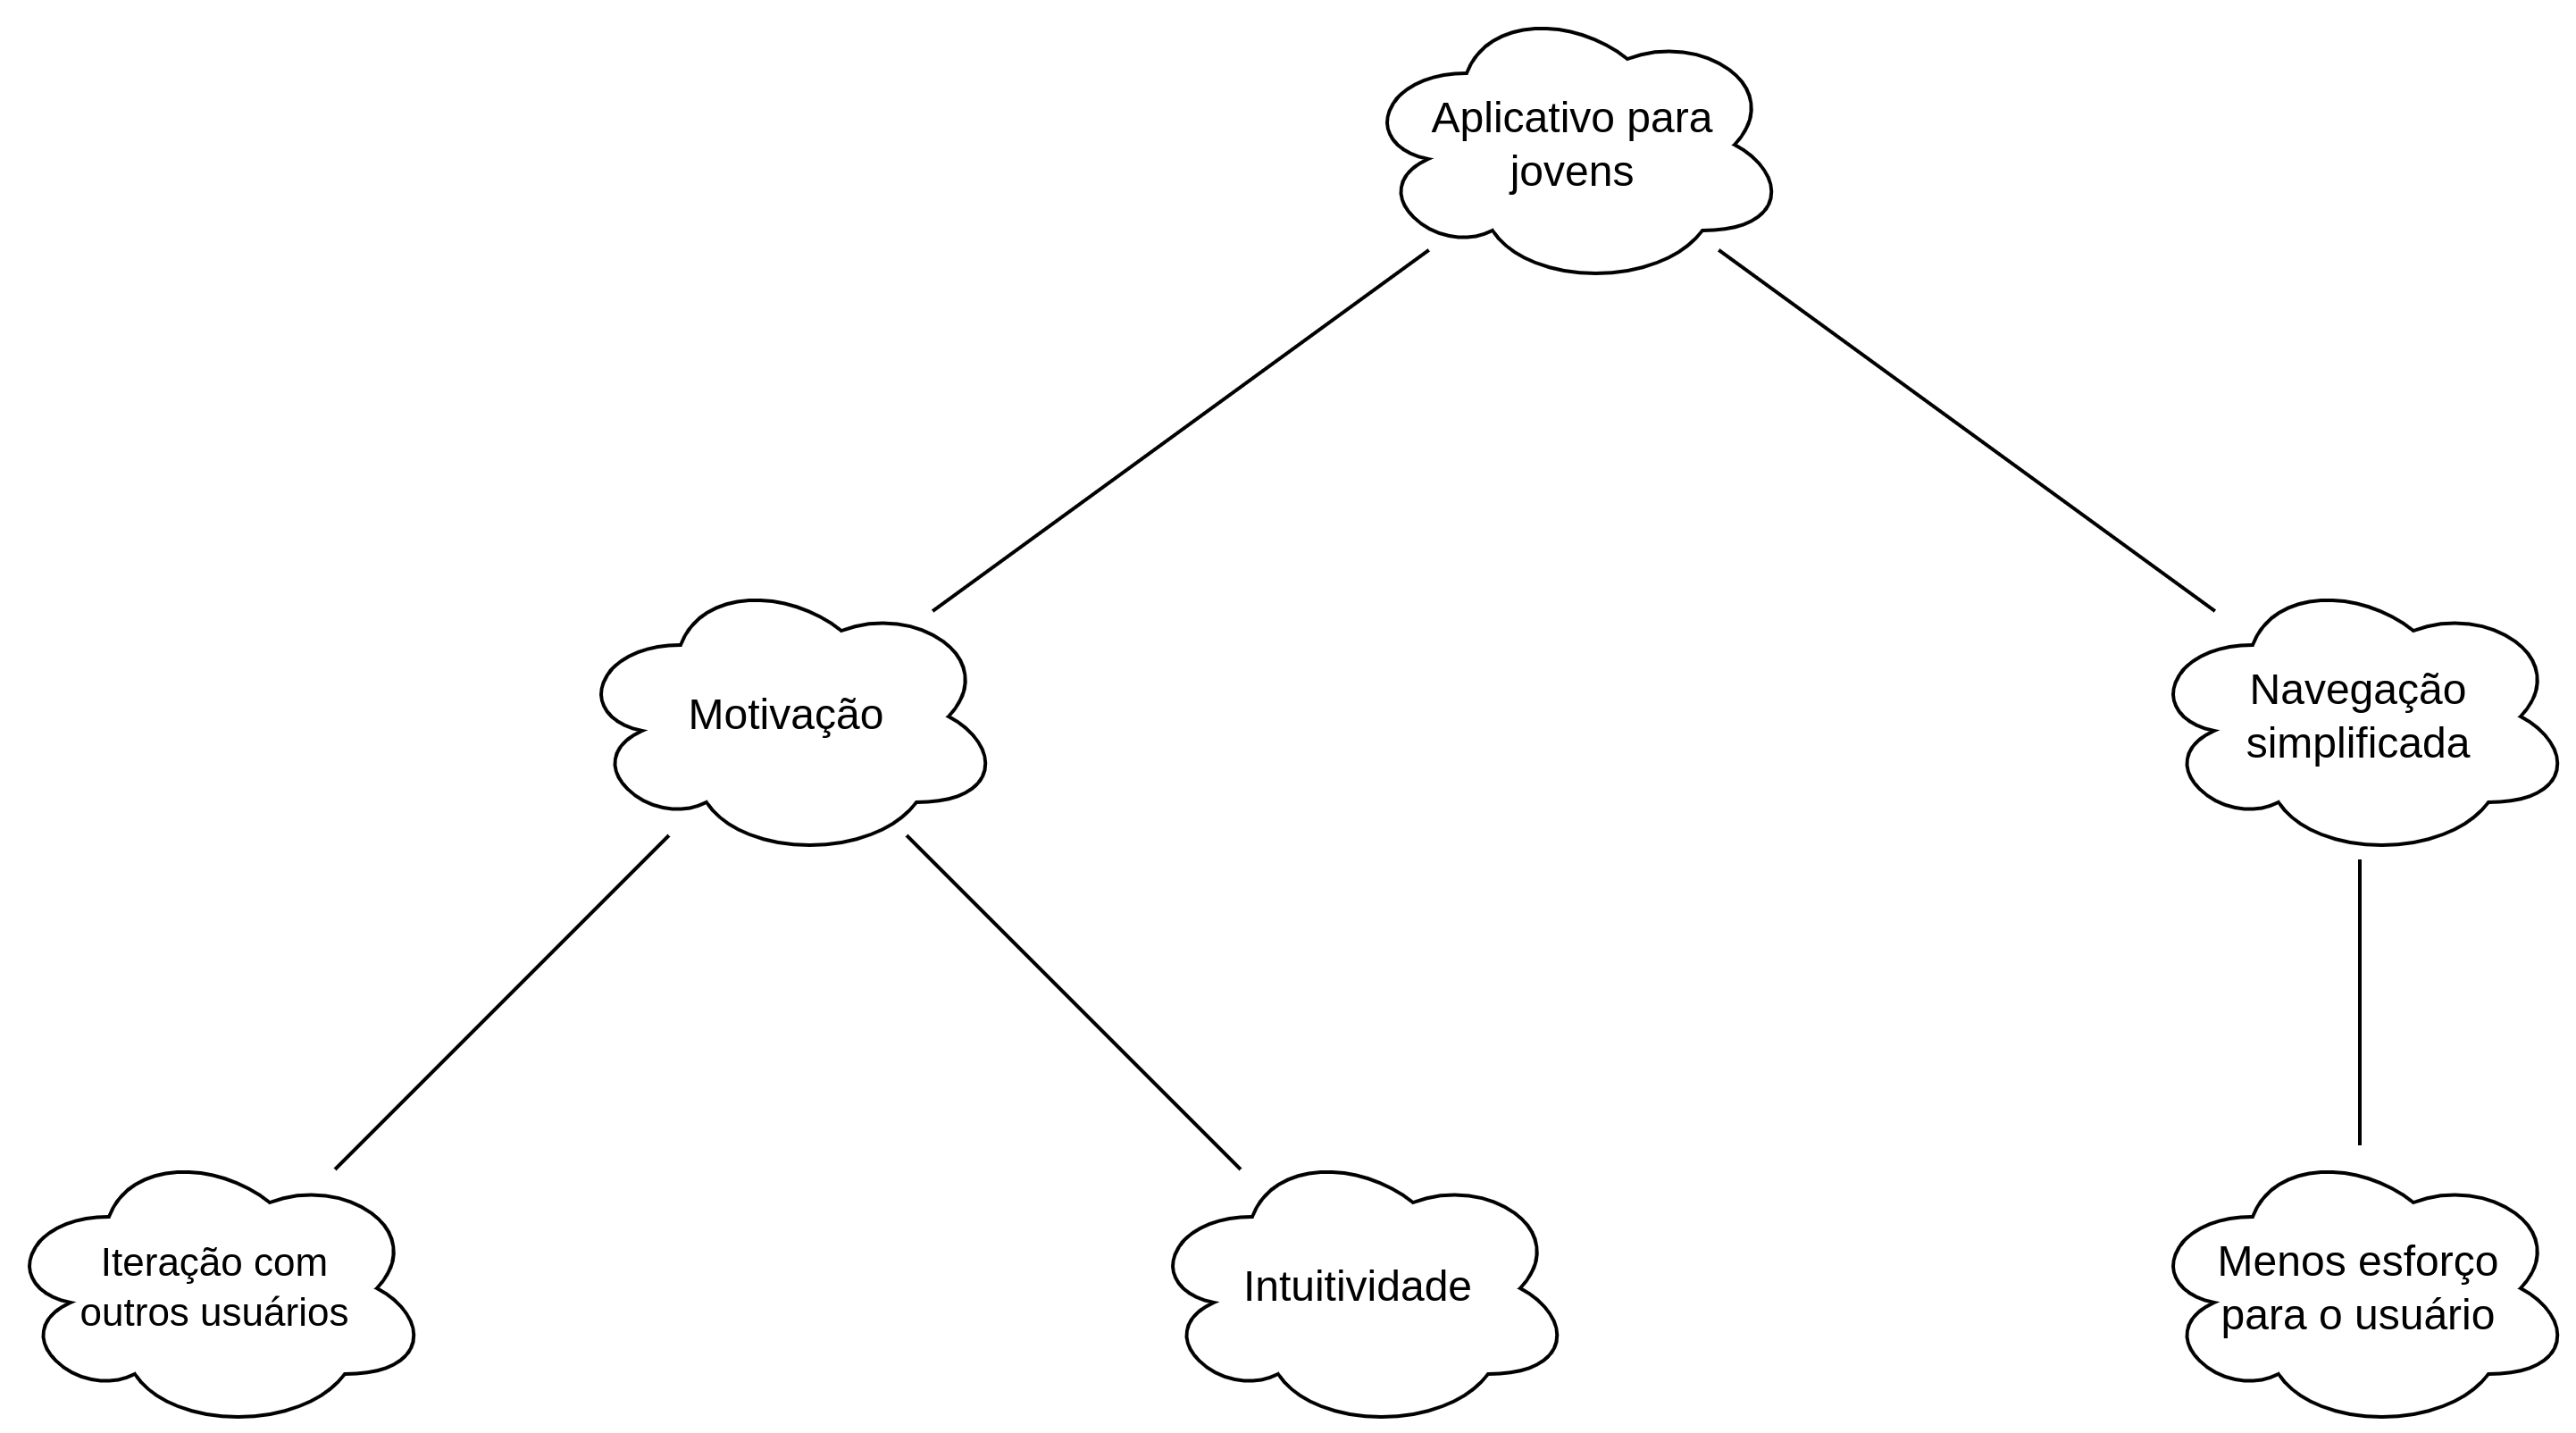
\includegraphics[scale=0.60]{figuras/Embasamento/nfr_adaptado.png}
        \legend{Fonte: Autores, 2022.}
    \end{center}
\end{figure}


\subsection{Léxicos}

\label{sec:lexicos}

O Léxico é definido como um conjunto de vocábulos de uma língua, dispostos em ordem alfabética e com as respectivas significações. Uma notação na modelagem de requisitos que usa a descrição de termos via léxico é o LAL (Léxico Ampliado da Linguagem). Trata-se de uma técnica que consiste em definir os símbolos de uma linguagem. Esses símbolos são descritos em \textbf{noções}\footnote{Significa o símbolo, é colocado no sentido denotativo da linguagem.} e \textbf{impactos}\footnote{Efeito/uso/ocorrência do símbolo na aplicação, que pode ser colocado no sentido conotativo da linguagem.} \cite{leite1993strategy}. Cada Léxico pode ser definido em somente um tipo, sendo eles:

\begin{itemize}
    \item Objetos: são aqueles que se relacionam com outros objetos;
    \item Verbos: são as ações, e
    \item Estados: são gerados a partir de ações (verbos).
\end{itemize}

Considerando um \textit{software} no domínio de um aplicativo \textit{mobile}, denominado Pró-Espécies Peixes, com a finalidade de aumentar a quantidade de informações disponíveis sobre as espécies de peixes no cerrado brasileiro, tem-se um exemplo de especificação de léxico, Tabela \ref{tab:lexico}, para o termo \textbf{Georreferência}, sendo esse do tipo \textbf{Objeto}.

\begin{quadro}[H]
\caption{Exemplo de léxico (Objeto)}
\centering
\begin{tabular}{L{0.15\textheight}|L{0.45\textheight}}
    \hline
    Nome & Georreferência \\ \hline
    Classificação & Objeto  \\ \hline
    Sinônimos & Geolocalização \\ \hline
    Noção & Funcionalidade de mapeamento e fornecimento da localização do usuário em um registro \\ \hline
    Impacto & A Georreferência, ou Geolocalização, permite fornecer a localização de onde ocorreu um determinado registro. \\ \hline
\end{tabular}
\legend{Fonte: Autores, 2022.}
\label{tab:lexico}
\end{quadro}

\section {Verificação}

\label{sec:verificacao}

Verificação consiste em uma etapa rigorosa do processo da Engenharia de Requisitos, onde os artefatos gerados na modelagem (Seção \ref{sec:modelagem}) são revisados. Essa etapa é essencial, pois no contexto do desenvolvimento de um \textit{software}, uma refatoração é mais custosa que a inspeção de um artefato previamente à implementação. São usadas diversas técnicas nesta etapa \cite{verification}, a depender da necessidade.

Nesse contexto, cabe uma ressalva. A etapa de análise, inerente na Engenharia de Requistos, envolve, principalmente, duas sub-atividades, sendo: Verificação e Validação. A verificação compreende analisar  se o \textit{software} está correto, conforme foi especificado/planejado/modelado. Já a validação analisa se o \textit{software}, obtido até o momento da análise, atende às expectativas do cliente.

É possível perceber que a validação é mais complicada de ser realizada, na Engenharia de Requisitos, visto que, nesta etapa do ciclo de vida, não há um incremento de \textit{software} avançado, tampouco um produto concluído. Quando muito, tem-se um protótipo ou um incremento de \textit{software} tido como uma prova de conceito. Portanto, costuma-se validar esse protótipo ou essa prova de conceito usando um grupo mais específico de \textit{Stakeholders}.

Em contrapartida, a verificação é comumente realizada na Engenharia de Requisitos, sendo utilizada, principalmente, a Técnica de Inspeção \cite{design_fagan} \cite{verification_MR}. Neste trabalho, a verificação foi priorizada.

\section{Priorização (MVP)}

\label{sec:priorizacao}

O MVP (\textit{Minimum Viable Product}) é definido como a versão mais simples de um produto que pode ser colocado para negociação. Determina quais são as funcionalidades mais importantes, que agregam mais valor ao produto para ele ser validado e efetivado pelo usuário final \cite{carolipaulo2018}. Faz-se uso deste conceito, no sentido da ferramenta elaborada auxiliar os Engenheiros de \textit{Software} na obtenção de um MVP, sendo esse orientado pelas boas práticas da Engenharia de Requisitos, mitigando problemas, mencionados no Capítulo \ref{chap:intro}.

Além disso, o MVP é usado para validar o retorno de determinado investimento, mesmo antes de o produto estar completamente finalizado, trazendo uma versão mais condensada, mas que, no entanto, já é suficiente para resolver o problema para o qual foi desenvolvido \cite{mvp}.

\section{\textit{House of Quality}}

\label{sec:house_of_quality}

\textit{House of Quality} ou Casa da Qualidade é um processo de planejamento sistemático, elaborado para compreender de forma explícita a “voz do cliente” no \textit{design} do produto. Esta pode ser vista como uma ferramenta gráfica para compreender e avaliar a relação entre as preocupações do cliente e as do desenvolvedor \cite{Howard_1}, conforme consta na Figura \ref{fig:hoq}.

\begin{figure}[]
    \begin{center}
        \caption{\textit{House of Quality} do Aplicativo Habitica}
        \label{fig:hoq}
        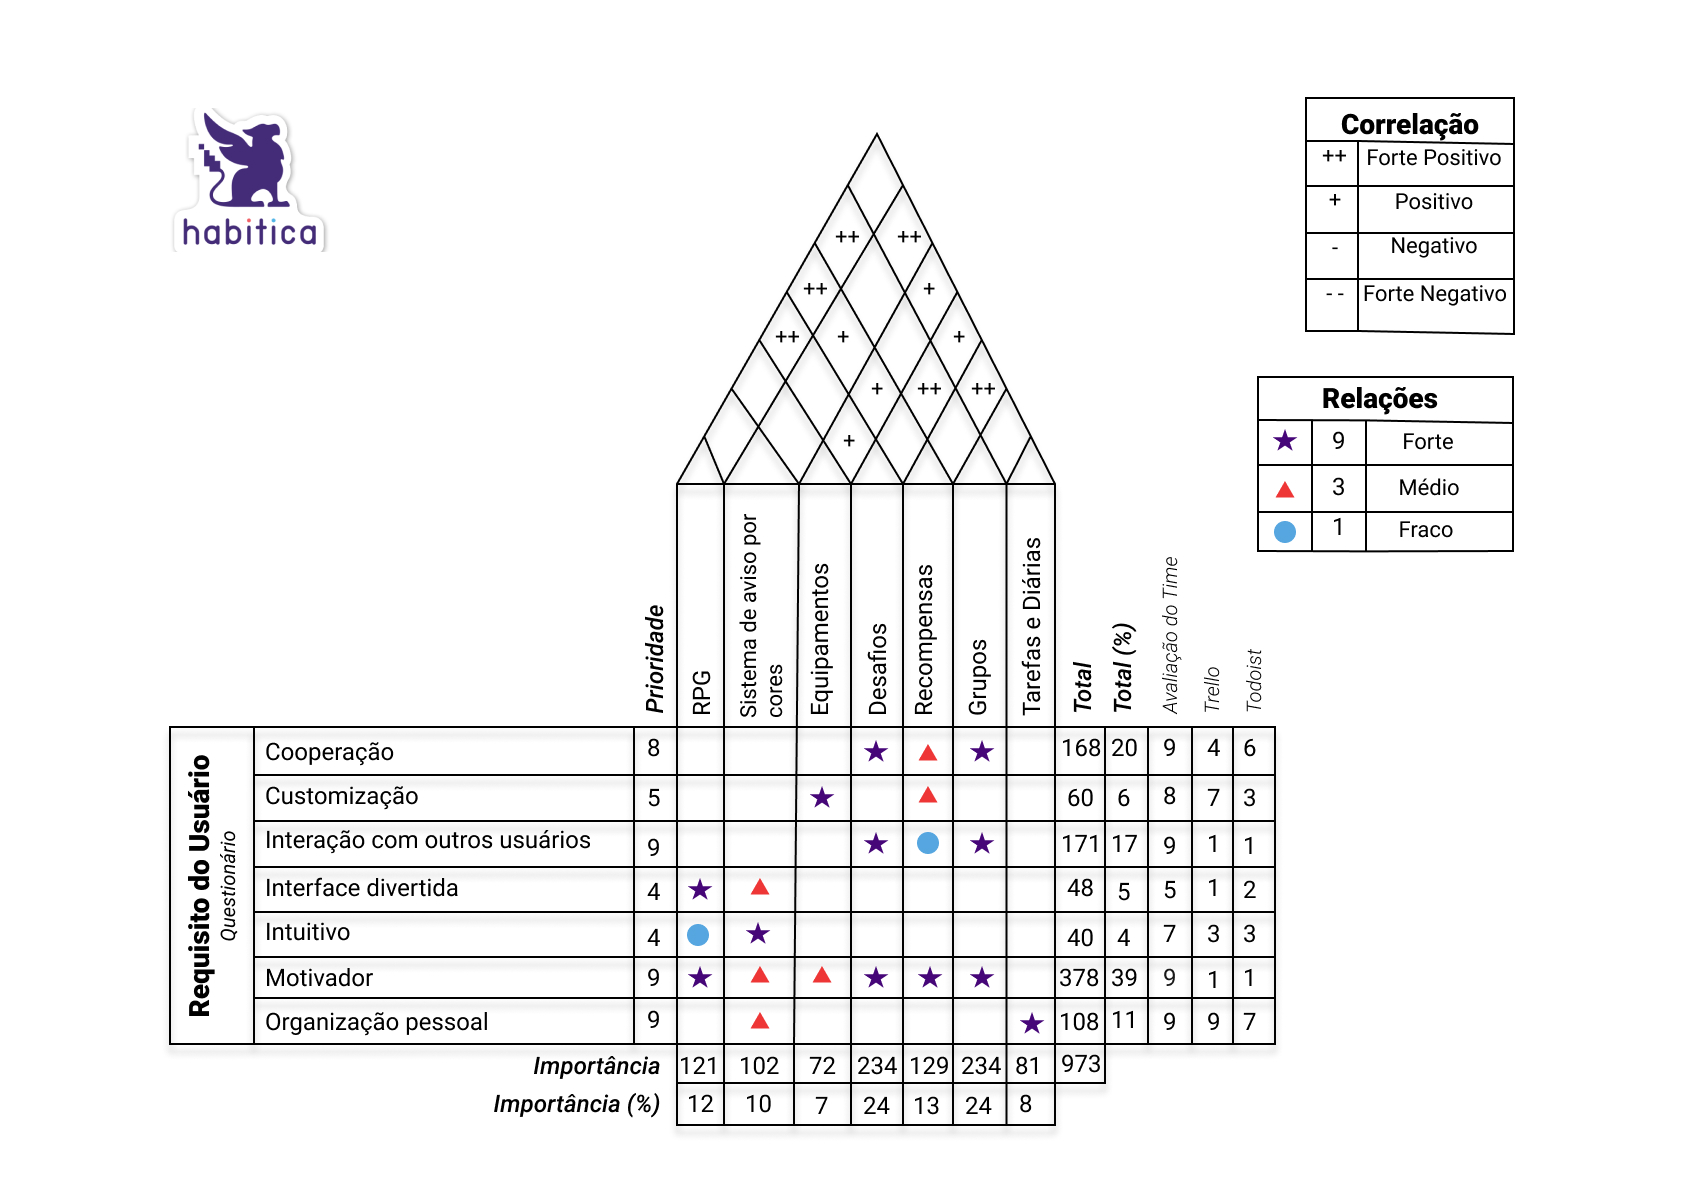
\includegraphics[scale=0.58]{figuras/referencial_teorico/HOQ.jpg}
        \legend{Fonte: Autores, 2022.}
    \end{center}
\end{figure}

Trata-se de um artefato composto por cinco partes, sendo elas:

\begin{itemize}
    \item No centro, são comparados os requisitos técnicos propostos com as necessidades do cliente, classificando sua relação;
    \item À direita, tem-se uma comparação dos concorrentes com relação ao produto da empresa, sobre as necessidades do cliente. Nela, é possível comparar os diferentes parâmetros dos concorrentes com o produto, bem como ter uma noção da qualidade do produto;
    \item À esquerda, têm-se as necessidades dos clientes acordadas com um peso de prioridade, para ser possível atender a maioria dessas necessidades;
    \item Na parte inferior, são comparados todos os requisitos dos produtos concorrentes com o da empresa, da mesma forma que com as urgências, e
    \item Na parte superior, têm-se as correlações dos requisitos técnicos, sendo onde são determinados os parâmetros conflitantes. Neles, que a equipe deve ponderar e descobrir o meio-termo no desenvolvimento.
\end{itemize}

\subsection{Grafos}

\label{sec:grafos}
Grafo é um ramo da matemática que estuda as relações entre os objetos de um determinado conjunto. Portanto, um Grafo $G$ é definido por um conjunto $V(G)$ de elementos denominados Vértices; um conjunto $E(G)$ de elementos chamados Arestas, onde cada aresta associa um ou dois vértices. A Figura \ref{grafo_1} mostra a representação de um grafo com os vértices $(A, B, C, D, E)$, suas respectivas arestas e os pesos $(3, 5, 9, 2, 1, 1, 6)$.

\begin{figure}[H]
    \begin{center}
        \caption{Exemplo de Grafo}
        \label{grafo_1}
        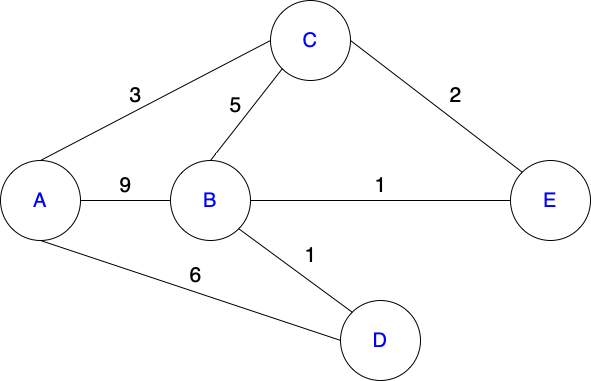
\includegraphics[scale=0.5]{figuras/referencial_teorico/Grafo.drawio.png}
        \legend{Fonte: Autores, 2022.}
    \end{center}
\end{figure}

Na computação, a lista de adjacências é uma das formas de representação de um grafo, existindo também a representação por matriz. Na lista de adjacências, têm-se as ligações de vértices e arestas com seus pesos respectivos. É uma maneira de codificar relações emparelhadas entre um conjunto de objetos. Consiste em uma coleção $V$ de nós e uma coleção $E$ de arestas, onde as arestas juntam dois nós \cite{Kleinberg+Tardos:06a}.

De acordo com \citeonline{prestes2016introduccao},  um grafo $G = (V, A)$, com $|V| = n$ e $|A| = m$, pode ser representado como uma matriz de adjacência. A matriz de adjacência é uma matriz $M = [m_{i,j}]$ simétrica  $n\times n$ que armazena o relacionamento entre os vértices do grafo. Cada entrada $m_{i,j}$ é igual a:

\[ m_{i, j} =
  \begin{cases}
    0,       & \quad \text{se } i \text{ não é adjacente a } j \\
    m,  & \quad \text{se } i \text{ é adjacente a } j \text{ com } i \neq j \\
    p, & \quad \text{se } i = j, p \text { é a quantidade de laços incidentes ao vértice } i
  \end{cases}
\]

\begin{figure}[H]
    \begin{center}
        \caption{Exemplo de um Grafo para a representação em Matrizes}
        \label{grafo_matriz}
        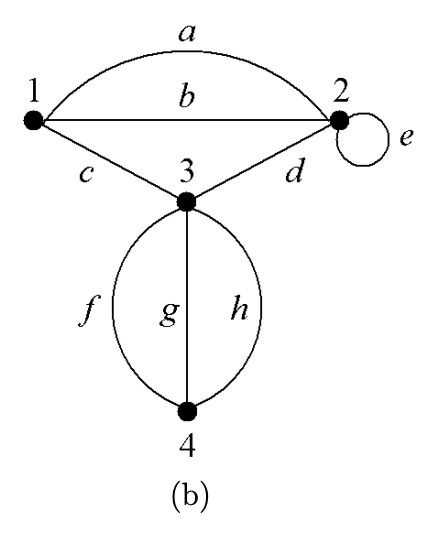
\includegraphics[scale=0.7]{figuras/Embasamento/grafo.png}
        \legend{Fonte: \cite{prestes2016introduccao}}
    \end{center}
\end{figure}

A Figura \ref{matriz_adj} representa uma matriz de adjacência para o Grafo exemplificado na Figura \ref{grafo_matriz}.

\begin{figure}[H]
    \begin{center}
        \caption{Matriz de adjacência para o Grafo da Figura \ref{grafo_matriz}}
        \label{matriz_adj}
        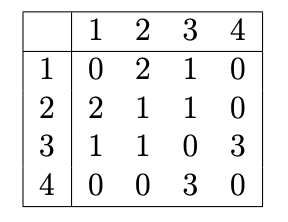
\includegraphics[scale=0.7]{figuras/Embasamento/matriz.png}
        \legend{Fonte: \cite{prestes2016introduccao}}
    \end{center}
\end{figure}


\subsubsection{Algoritmo de Menor Caminho}

\label{sec:ssp}

O Algoritmo de Menor Caminho consiste em calcular, para cada vértice $V$, a menor distância de $S$ para $V$, ou seja, a menor soma possível de pesos de arestas que formem um caminho de $S$ para $V$, onde $S$ e $V$ são vértices dentro de um grafo $G$. Os Algoritmos de \textit{Dijkstra} e \textit{Bellman-Ford} são os mais conhecidos para realizar o cálculo da menor distância entre dois vértices \cite{even2011graph}.

No caso do presente trabalho, foi utilizado o Algoritmo de Dijkstra para se calcular o menor caminho entre as relações de requisitos funcionais e não funcionais para que se tenha o Produto Mínimo Viável, na sua versão preliminar. Foi escolhido esse algoritmo por não haver pesos negativos na modelagem do grafo do relacionamento entre os requisitos.

\section{Resumo do Capítulo}

\label{sec:resumo_embasamento}

Neste capítulo, foram apresentados os principais conceitos que servem como base para o entendimento do contexto do trabalho desenvolvido, no caso, o \textit{iFlow}: uma ferramenta que oferece apoio ao processo de Engenharia de Requisitos, objetivando a construção de um MVP.

Para a apresentação desses conceitos, fez-se necessária uma breve explicação sobre cada etapa do processo de Engenharia de Requisitos, fazendo correlação com a ferramenta desenvolvida. O grande intuito é contextualizar o processo e os artefatos gerados em cada etapa.

Em seguida, tem-se uma explanação concreta da Engenharia de Requisitos e sua importância no processo de construção de um produto de \textit{software}, bem como diversas etapas essenciais neste processo, de modo a oferecer um panorama geral a respeito da Engenharia de Requisitos. Em seguida, foram apresentadas as principais etapas no processo de Engenharia de Requisitos, sendo elas: Pré-rastreabilidade; Pós-rastreabilidade; Elicitação; Modelagem; Verificação; e Priorização.

Por fim foram explorados conceitos importantes no contexto do desenvolvimento deste trabalho que foram o \textit{House of Quality} e os Grafos.